%%
%% Berliner Hochschule für Technik -- Abschlussarbeit
%%
%% Hauptdokument
%%
%% 23.01.09 Tschirley V.01 Beuth Hochschule
%% 26.08.21 Tschirley V2.0 Umbenennung zur Berliner Hochschule für Technik
%%
%%%%%%%%%%%%%%%%%%%%%%%%%%%%%%%%%%%%%%%%%%%%%%%%%%%%%%%%%%%%%%%%%%%%%
\documentclass[11pt, a4paper]{book}
%\documentclass[11pt, a4paper, oneside]{book}
%% Übersetzen als Entwurf
\usepackage[entwurf]{bhtThesis}
%% Übersetzen für die Abgabe
%\usepackage[abgabe]{bhtThesis}
\typeout{BHT-Abschlussarbeit V2.0 26.08.21 S.Tschirley}

\usepackage{blindtext}   %für Blindtext in Kapitel 2
\usepackage{listings}
\lstset{ 
  literate={ö}{{\"o}}1
           {ä}{{\"a}}1
           {ü}{{\"u}}1
           {Ö}{{\"O}}1
           {Ä}{{\"A}}1
           {Ü}{{\"U}}1
           {ß}{{\ss}}1
}
\usepackage{hyperref}

%%
%% Es folgen einige Zusätze, die in Kapitel 1 beschriben sind. 
%% Alles was nicht notwendig ist, kann auskommentiert werden
%%
\usepackage{trsym}
%\usepackage{showkeys}
\usepackage{bytefield}
\usepackage{svg}

%%
%% Pfad zu den Bildern
%%
\graphicspath{
  {pictures/},
  {einleitung/pictures},
  {kapitel1/pictures/},
  {kapitel2/pictures/}
}

%%
%% Einbinden persönlicher macros 
%%
%
% Persönliche Macros
%
%

% Macros für Formeln
\newcommand{\jw}{j\omega}

% Begriffe

\newcommand{\OPV}{Operations\-ver\-stär\-ker}



%% Message
\typeout{-----------------------------------------------------------}
\typeout{----> main.tex ---- Zentrales Dokument---------------------}
\typeout{-----------------------------------------------------------}

\version{0.1$\alpha$}    % word im Entwurf auf der Titelseite vermerkt
\datum{\today}
%%
%% Titel, Autor und Betreuer
%%
\fachbereich{VI -- Informatik und Medien} 
\studiengang{Medieninformatik Online}
\thesistyp{Masterarbeit} 
\autor{Denis Renning}
%\edvnr{123 456}
\titel{Web Application Firewalls und Machine Learning} 
\untertitel{Migration und Erweiterung am Beispiel}
\betreuerFeld{
  \begin{tabular}{lr}
    \multicolumn{2}{l}{\textbf{Gutachter}}\\
    Prof.~Dr.~S.~Edlich & Berliner Hochschule für Technik\\
    Prof.~Dr.~S.~Haschemi& Berliner Hochschule für Technik
  \end{tabular}
}

%%\renewcommand{\baselinestretch}{1.05} 
\begin{document}
\pagestyle{fancy}

%%
%% Berliner Hochschule für Technik --  Abschlussarbeit
%%
%% Titelseiten und Erklärungen 
%%
%%%%%%%%%%%%%%%%%%%%%%%%%%%%%%%%%%%%%%%%%%%%%%%%%%%%%%%%%%%%%%%%%%%%%

\maketitle
\clearpage
%\thispagestyle{empty}
% Rueckseite (leer)
%% 
~
\newpage

%%
%% Abstract
%%
%%%%%%%%%%%%%%%%%%%%%%%%%%%%%%%%%%%%%%%%%%%%%%%%%%%%%%%%%%%%%%%%%%%%%


\section*{Kurzfassung}
Die Kurzfassung gibt  ein kurzes und prägnantes Bild der  gesamten Arbeit. Sie soll
den  Leser  neugierig  machen  und  klarmachen,  was  zu  erwarten  ist.  Erreichte
Ergebnisse werden kurz umrissen.

%% eof

%%
%% Abstract
%%
%%%%%%%%%%%%%%%%%%%%%%%%%%%%%%%%%%%%%%%%%%%%%%%%%%%%%%%%%%%%%%%%%%%%%


\section*{Abstract}
Bachelor  and Master-Thesises usually  are often  written in  german. Nevertheless,
their content may be intersting for people  being not able to read german. In order
to  awaken their interest  in this  topic, an  abstract in  english is  given.  The
experimental results and analysis are shown in short

%% eof

\clearpage

%\ifthenelse{\boolean{@entwurfset}}
%    {

%    }
%    {
%      ~
%      \newpage
%      \vfill
%      \section*{Aufgabenblatt -- durch Original austauschen !!!}
%      \vfill
%      \clearpage
%      ~
%      \newpage
%    }
\vspace{10ex}
\section*{Erklärung}
Ich  versichere, dass  ich diese  Abschlussarbeit ohne  fremde  Hilfe selbstständig
verfasst und  nur die  angegebenen Quellen und  Hilfsmittel benutzt  habe. Wörtlich
oder dem  Sinn nach  aus anderen  Werken entnommene Stellen  sind unter  Angabe der
Quellen kenntlich gemacht.
\vspace{10ex}\\

\hrule
{\small{Datum}}\hfill{\small{Unterschrift}}


\pagenumbering{roman}
\tableofcontents
\listoffigures




\pagenumbering{arabic}
%%%%%%%%%%%%%%%%%%%%%%%%%%%%%%%%%%%%%%%%%%%%%%%%%%%%%%%%%%%%%%%
%% Die Kapitel der Arbeitw

%Einfuehrung (insgesamt ca. 5 Seiten)
%  Das grosse Problem
%  Ziel der Arbeit (oder das kleine machbare Problem)
%  Methodik (1 Seite)
%  Gliederung und Aufbau (0,5 Seiten)
%%%
%% Berliner Hochschule für Technik --  Abschlussarbeit
%%
%% Kapitel 1
%%
%%

\chapter{Erster Abschnitt}

Der   erste   Abschnitt   soll   eine  \index{Bedienungsanleitung}   sein.   Dieses
Beispieldokument einer  Abschlussarbeit ziegt alle  Möglichkeiten auf, die  mit dem
style  \texttt{bhtThesis.sty} realisiert  werden können.  Das bedeutet  nicht, dass
alle Funktionalitäten zwingend in allen Arbeiten eingesetzt werden müssen.

\section{Voraussetzungen}
Dieses  Dokument verwendet natürlich  auch andere  \LaTeX-Pakete. Auf  Ihrem System
sollten vorhanden sein:

\begin{itemize}
\item \texttt{ifthen}: Interne Verwendung für Abfragen
\item \texttt{graphicx}: 
  Einbinden von Grafiken
\item \texttt{array, tabularx}                  
  Tabellenerweiterungen
\item \texttt{multicol}                       
  Tabellenerweiterungen
\item \texttt{xcolor}                           
  Farbgebung im Textsatz
\item \texttt{siunitx}
  Einheiten beim Namen nennen
\item \texttt{changebar}
  Changbars am Rand zur Hilfe bei Korrekturen und Neuerstellugen
\item \texttt{fancyhdr} Seitenlayout
\item \texttt{listings} Paket für das  Einbinden von Quelltexten. Diese Paket kennt
  sehr  viele  Optionen  und  Einstellungsmöglichkeiten. Die  für  dieses  Dokument
  verwendeten   \LaTeX-Code-Fragmente   werden   ebenfalls   damit   gesetzt,   die
  Einstellungen stehen in Abschnitt \ref{ss.bht.listings}.
\end{itemize}

Alle diese Pakete werden mit einer Dokumentation ausgeliefert, in denen die genauen
Funktionalitäten  erklärt werden.   Diese Dokumentation  wird bei  der Installation
bereits  im  Dateisystem  abgelegt.   Bei  Mik\TeX-Systemen  ist  dies  der  Ordner
\verb|c:\textmf\doc\latex|.

%%
%%
%%
\section{Optionen des Styles \texttt{bhtThesis.sty}}
\lstset{language=[LaTeX]TeX,
 	basicstyle=\ttfamily\color{black}\small,
 	keywordstyle=\bfseries\color{bhtBlue},
 	identifierstyle=\color{black}, 
 	commentstyle=\color{gray}\textsl,
}
Die übergeordnete Dokumentenklasse ist \texttt{book}, das bedeutet
\begin{itemize}
\item Die Gliederungsebene \emph{Kapitel} (\texttt{chapter}) existiert.
\item Der Druck ist zweiseitig und als Folge davon
\item starten alle Kapitel auf der ungeraden Seite, im aufgeschlagenen Buch auf der
  rechten Seite. Sollte das nicht gewünscht sein, so kann  man auf einseitige
  Ausgabe bestehen mit
\begin{lstlisting}
  \documentclass[11pt, a4paper, oneside]{book}
\end{lstlisting}
  Die Datei \texttt{titelseiten.tex} ist dann manuell anzupassen.
\end{itemize}

Das Dokument kann mit
\begin{lstlisting}
  \usepackage[entwurf]{bhtThesis}
\end{lstlisting}
als Entwurf übersetzt werden. Dies ist auch die Voreinstellung. Hier werden
Revisionsbaken (vergl.~\ref{ss.bht.rev}) dargestellt, die Versionsnummern und das
Datum der letzten Übersetzung auf der Titelseite ausgegeben und das Wasserzeichen
gedruckt. Alle Randnotizen werden gesetzt.

Die Option
\begin{lstlisting}
  \usepackage[abgabe]{bhtThesis}
\end{lstlisting} 
schaltet alles dies aus, es erscheinen keine Randnotizen.

%%
%%
%%
\section{Funktionen}

\subsection{Farben}
Der     Style     \texttt{bhtThesis.sty}      definiert     die     Hochschulfarben

\textcolor{bhtGray}{bhtGray \Large{\ding{110}}},
\textcolor{bhtBlue}{bhtBlue                                    \Large{\ding{110}}},
\textcolor{bhtTurquoise}{bhtTurquoise                            \Large{\ding{110}}},
\textcolor{bhtYellow}{bhtYellow  \Large{\ding{110}}} und  \textcolor{bhtRed}{bhtRed
  \Large{\ding{110}}}.\\
Mit   dem    Kommando   \verb|\textcolor{bhtBlue}{einzelne    Textpassagen}|   sind
\textcolor{bhtBlue}{einzelne  Textpassagen}  einfärbbar.    Dies  sollte  aber  mit
Bedacht geschehen, zuviel Farbe wird schnell zur Belästigung.

\subsection{Umgebung \texttt{neu}}\label{ss.bht.rev}

Die Umgebung 
\lstset{language=[LaTeX]TeX,
 	basicstyle=\ttfamily\color{black}\small,
 	keywordstyle=\bfseries\color{bhtBlue},
 	identifierstyle=\color{black}, 
 	commentstyle=\color{gray}\textsl,
}
\begin{lstlisting}
  \begin{neu}
    Hier folgt ein Absatz, der neu eingefügt ist.
    Der soll unbedingt gelesen werden. ß
  \end{neu}
\end{lstlisting}
erzeugt einen Revisionsbalken und einen Hinweis:

\begin{neu}
    Hier folgt ein Absatz, der neu eingefügt ist. 
    Der soll unbedingt gelesen werden. 
\end{neu}

Die Revisionsbalken werden in  Extradateien der Endung \texttt{*.cb*} verwaltet. Es
ist mehrfaches übersetzen  nötig.  Die finale Version mit  der Option \verb|[abgabe]|
hat keine Markierungen, auch der Hinweistext entfällt dann.

\subsection{Randnotizen}
Für  den Fall,  das  während  des Schreibens  kleine  Erinnerungsnotizen zu  machen
\anno{Abschnitt    muss   überarbeitet    werden}   sind,    kann    das   Kommando
\verb|\anno{Abschnitt...werden}| eingesetzt werden.  Diese können im laufenden Text
untergebracht werden und erscheinen in der Zeile, wo sie erzeugt wurden. Die Option
\verb|[abgabe]| schaltet die Randnotizen aus.

\subsection{Einstellung von \texttt{listings}}\label{ss.bht.listings}

\lstset{language=[LaTeX]TeX,
 	basicstyle=\ttfamily\color{black}\small,
 	keywordstyle=\bfseries\color{bhtBlue},
 	identifierstyle=\color{black}, 
 	commentstyle=\color{gray}\textsl,
 }

Die \LaTeX\-Code-Fragmente werden mit den folgenden Voreinstellungen gesetzt:
\begin{lstlisting}
  \lstset{language=[LaTeX]TeX,
 	basicstyle=\ttfamily\color{black}\small,
 	keywordstyle=\bfseries\color{bhtBlue},
 	identifierstyle=\color{black}, 
 	commentstyle=\color{gray}\textsl,
        }
\end{lstlisting}

Es sind weit  mehr Einstellungen möglich, hier sei auf  die Dokumentation zum Paket
verwiesen.  Die   Einstellungen  für  das   Paket  erfolgen  nicht  in   der  Datei
\texttt{bhtThesis.sty}.

Für Code in C++ sähe der Parametersatz für \texttt{\textbackslash lstset\{\}} so aus
\begin{lstlisting}
\lstset{language=C++,
  basicstyle=\ttfamily\color{black}\small,
  keywordstyle=\color{bhtBlue}\bfseries,
  commentstyle=\color{bhtGray}\slshape,,
  identifierstyle=\color{black}}
\end{lstlisting}

Das Resultat ist dann das folgende:

\lstset{language=C++,
  basicstyle=\ttfamily\color{black}\small,
  keywordstyle=\color{bhtBlue}\bfseries,
  commentstyle=\color{bhtGray}\slshape,,
  identifierstyle=\color{black}}
\begin{lstlisting}
class Mitarbeiter
{
  private:              
    float		gehalt;       // sollte man haben
    int			krankenkasse; // das auch
    int			steuerklasse; // das will man nicht

  public:
    
    virtual float	berechneLohnsteuer();
    float		berechneKrankenversicherung();
    float		berechneRentenversicherung();
};

class Vollzeitangestellter : public Mitarbeiter
{
  public:
    float		berechneLohnsteuer();

};

class Teilzeitangestellter : public Mitarbeiter
{
    float		berechneLohnsteuer();
};
\end{lstlisting}

Verwendet    man   verschiedene    Sprachen    in   einem    Dokument,   so    muss
\texttt{\textbackslash  lstset\{\}}  \textbf{vor}   jedem  neuen  Codefragment  neu
angepasst werden.

Problematisch sind Umlaute  in Quellen, die zum Beispiel  in Kommentaren eingesetzt
werden. Diese werden nicht ohne weiteres erkannt. Dies kann aber geklärt werden, in
dem man  die Buchstaben der  Umlaute dem \TeX-Quellcode  zuweist, am besten  in der
Präambel des Dokuments.

\lstset{language=[LaTeX]TeX,
 	basicstyle=\ttfamily\color{black}\small,
 	keywordstyle=\bfseries\color{bhtBlue},
 	identifierstyle=\color{black}, 
 	commentstyle=\color{gray}\textsl,
        }
\begin{lstlisting}
\lstset{ 
  literate={ö}{{\"o}}1
           {ä}{{\"a}}1
           {ü}{{\"u}}1
           {Ö}{{\"O}}1
           {Ä}{{\"A}}1
           {Ü}{{\"U}}1
           {ß}{{\ss}}1
}
\end{lstlisting}


\subsection{Literaturverzeichnisse mit bib\TeX}
Das Literaturverzeichnis kann automatisch mit bib\TeX erstellt werden. 

Für   dieses  Dokument   befinden   sich  alle   Literaturstellen   in  der   Datei
\texttt{bhtThesis.bib}.  Die Einträge für  zu zitierende  Werke haben  die folgende
Form:
 \lstset{language=[LaTeX]TeX,
 	basicstyle=\ttfamily\color{black}\small,
 	keywordstyle=\bfseries\color{bhtBlue},
 	identifierstyle=\color{black}, 
 	commentstyle=\color{gray}\textsl,
        }
 \begin{lstlisting}
@book{albach.GdE2,
  author={Manfred Albach},
  title={{Grundlagen der Elektrotechnik 2}},
  publisher={Pearson Studium},
  year={2005}
}
 \end{lstlisting}

Damit das problemlos funktioniert, muss die Datei \texttt{bhtThesis.bib} im
Dateisystem auffindbar sein. Hierzu wird beispielsweise auf einem Linux-System die
Umgebungsvariable \texttt{\$BIBINPUTS} gesetzt zu
\begin{lstlisting}
  export BIBINPUTS=/home/tschirley/bibinput
\end{lstlisting}

Soll  dieses  Werk  referenziert  werden,  so  geschieht  dies  durch  den  Eintrag
\verb|\cite{albach.GdE2}|, wodruch der entsprechende  Verweis erzeugt wird, wie zum
Beispiel hier: \cite{albach.GdE2}.

Nun ist mehrmaliges übersetzen des  Dokuments notwendig. Um das fertige Dokument zu
erhalten muss sowohl \LaTeX\ als auch bib\TeX\ aufgerufen werden:
\begin{lstlisting}
localhost:> pdflatex main.tex
localhost:> bibtex main
localhost:> pdflatex main.tex
localhost:> pdflatex main.tex
\end{lstlisting}
Idealerweise  verwendet man \texttt{make}  und das  mitgelieferte \texttt{makefile}
für diese Aufgaben oder schreibt ein shellscript.

Prinzipiell  kennt  bib\TeX\  mehrere  Literaturtypen,  die  sich  dann  durch  die
notwendigen  Felder unterscheiden.   Für weiterführende  Informationen sei  auf die
zahlreichen  Dokumentation  von  bib\TeX\  wie  zum  Beispiel  \cite{bibTeX.manual}
verwiesen.

Ob im Text Zahlen (z.~.B. so [2]) auftauchen oder ganze Autorennamen ist sicher
individuell anders gewünscht. Das Mittel der Einstellung ist der
\texttt{bibliographystyle} im Zentraldokument. Gleichmaßen wird der Satzx des
Leiteraturverzeichnisses an sich verändert. Hier sind beispielsweise möglich:
\begin{itemize}
\item \texttt{ieeetr}
\item \texttt{natbib}
\item \texttt{apalike}
\end{itemize}

\section{Hinweise}

\subsection{Formelsatz}
Fu den Formelsatz stehen alle  Werkzeuge zur Verfügung. Die Pakete \texttt{amsmath}
und \texttt{amssymb}  werden eingebunden, so dass auch  mehrzeilige Formeln setzbar
sind:

Die Umgebung \texttt{multline} liefert dies:
\begin{multline}
        g_i(t) = \left( \frac 1 4 \,P_{k,i}\,F \left[ \underbrace{
                \sum_{n=\pm 1} e^{\,jn[(\omega_0+\omega_1)t + \varphi_i]} }_{\approx 0}
                \sum_{n=\pm 1} e^{\,jn[(\omega_0-\omega_1)t + \varphi_i]} \right] 
                \ast h_i(t) \right) 
                \\ \cdot
                \frac 1 2 \,Q_{k,i} \sum_{n=\pm 1} 
                 e^{\,jn(\omega_0 t + \varphi_i + \Delta\varphi_i)}
\end{multline}

\texttt{align} richtet am Gleichheitszeichen aus, auch über eingesetzte Textzeilen
hinweg: 
\begin{align}
    P_V &= \int\limits_0^T\;u(t)\cdot i(t)\;dt\\
\intertext{und das ist beim Transistor}
    P_V &= \int\limits_0^T \; u_{CE}(t)i_C(t)\;+\; u_{BE}(t)i_B(t)\;dt
\end{align}

\subsection{Grafiken}
Das   Paket   \texttt{graphicx}   bietet   die  Möglichkeit,   komfortabel   Bilder
einzubinden.  Das Kommando \verb|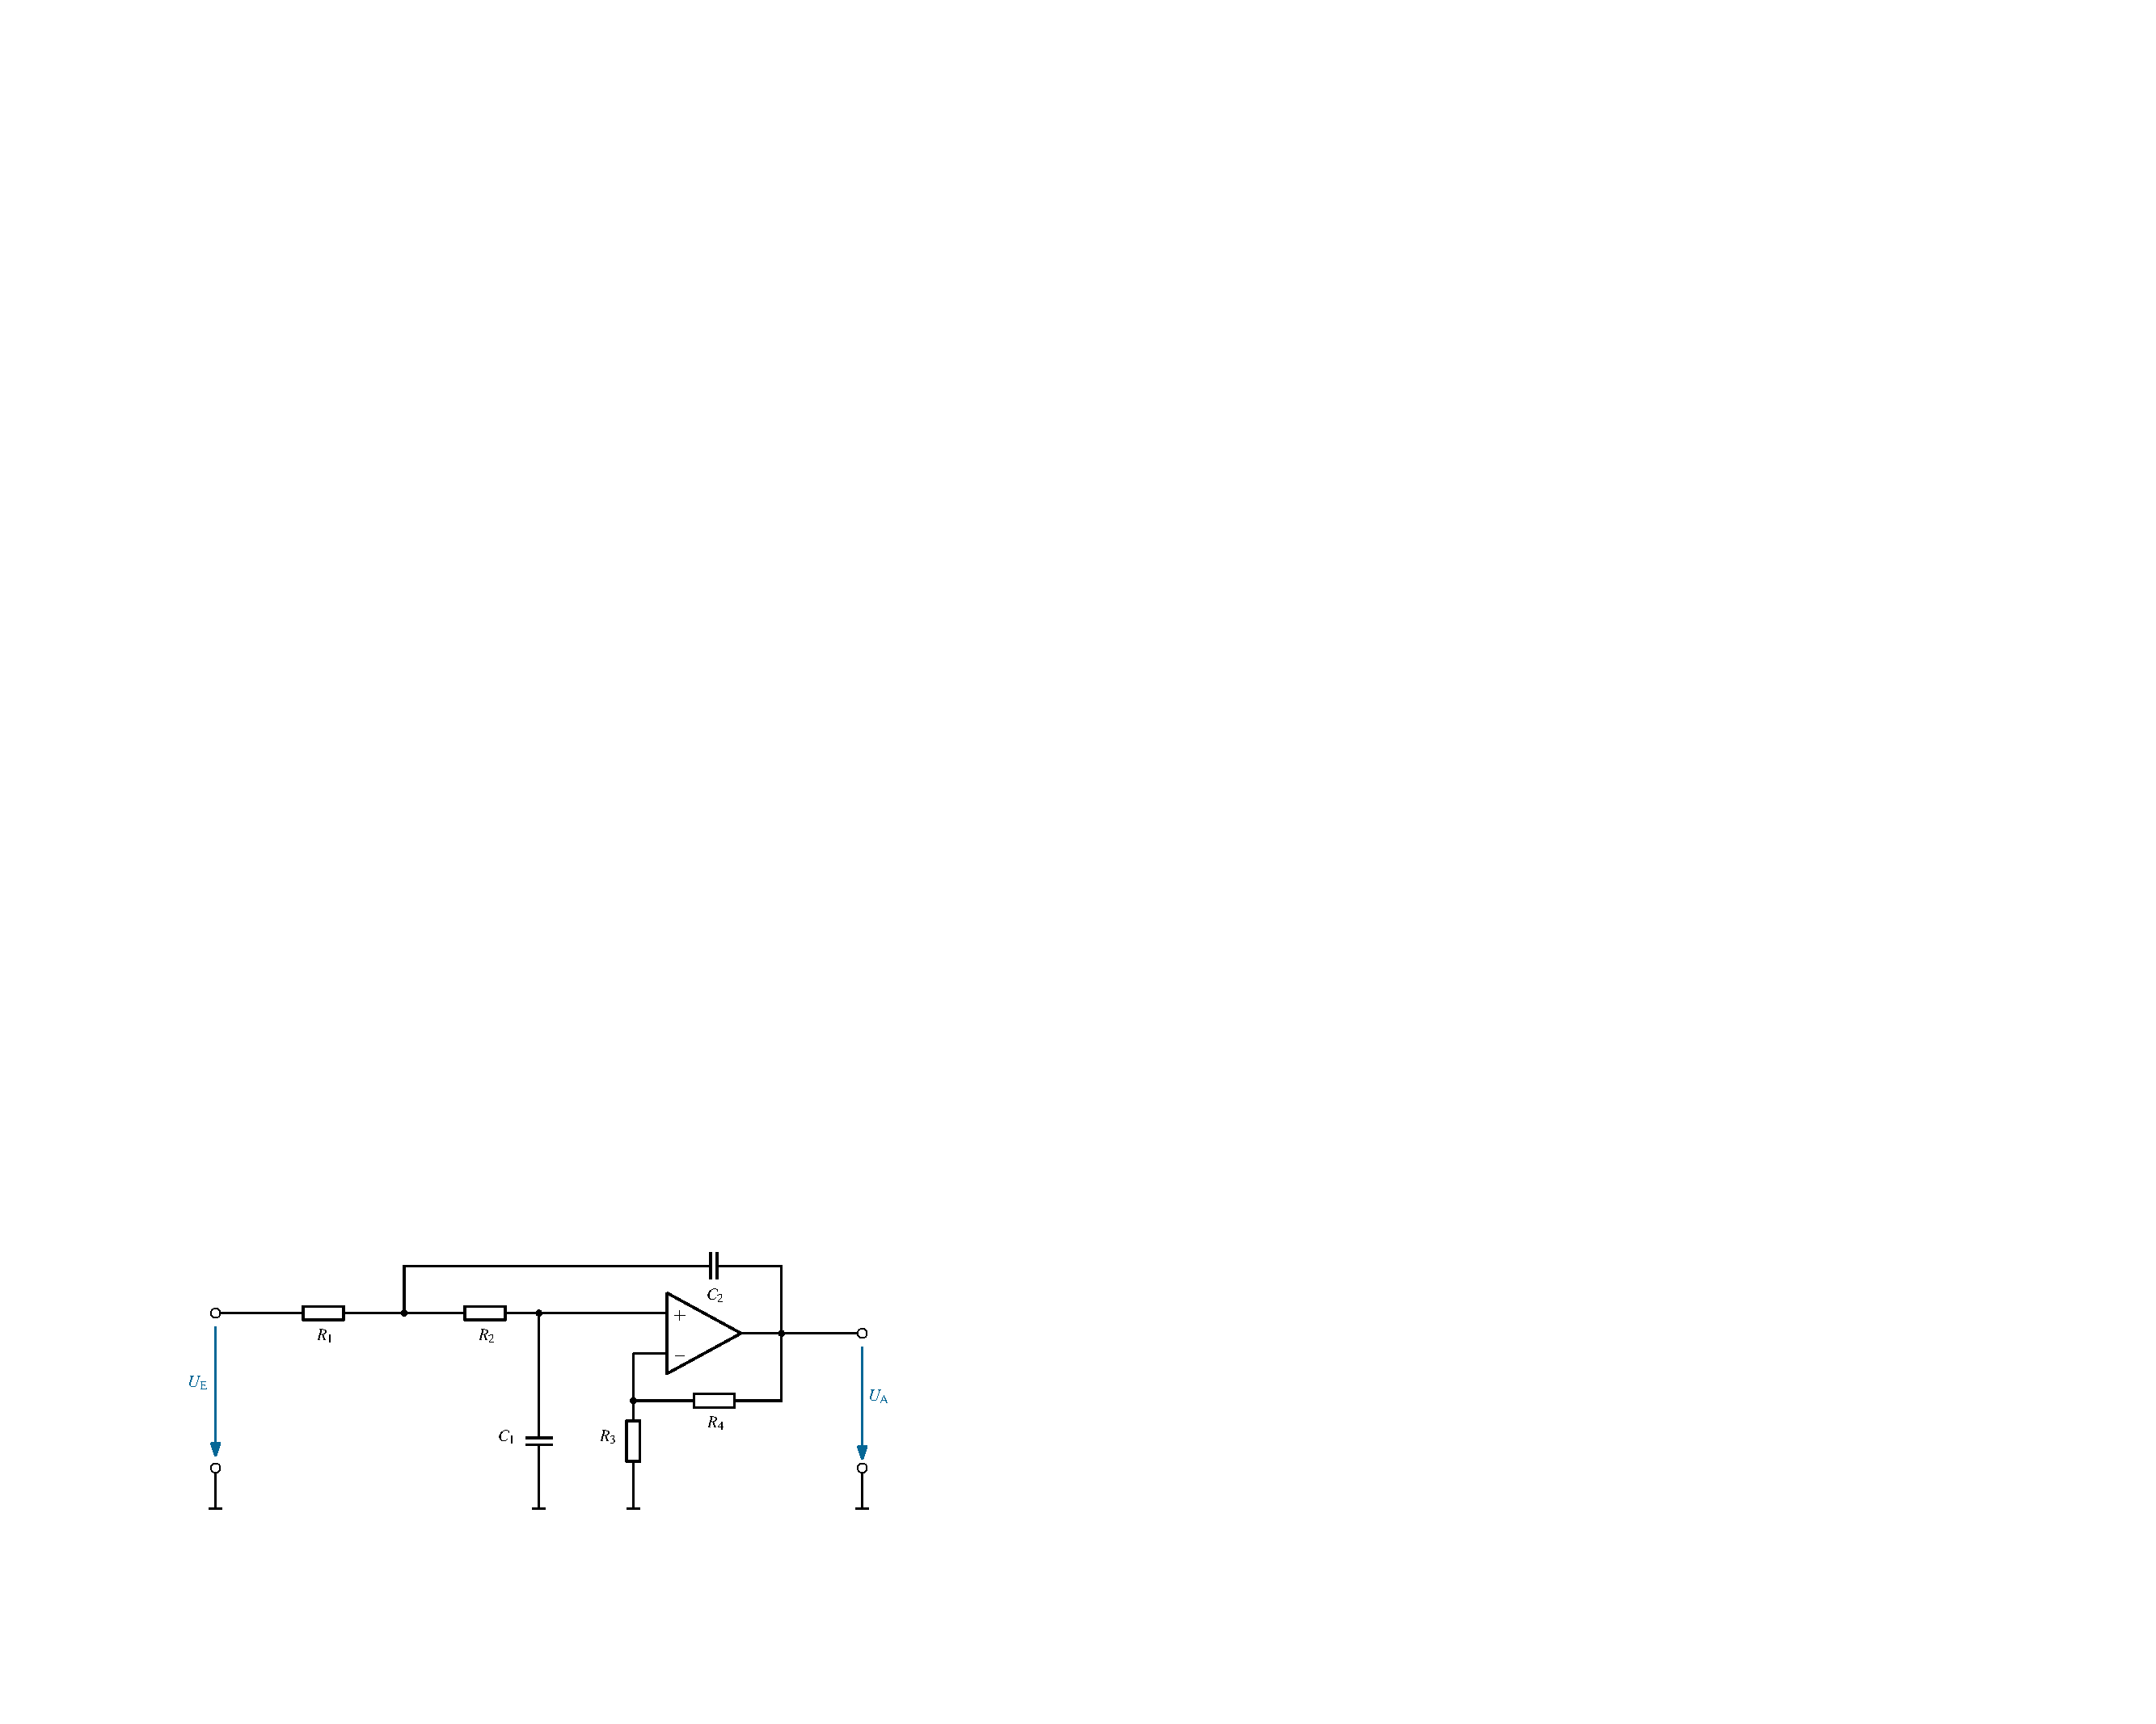
\includegraphics[scale=1]{schaltbild}|  erzugt ein
Bild an der Stelle des Aufrufes:

\begin{lstlisting}
  \begin{center}
    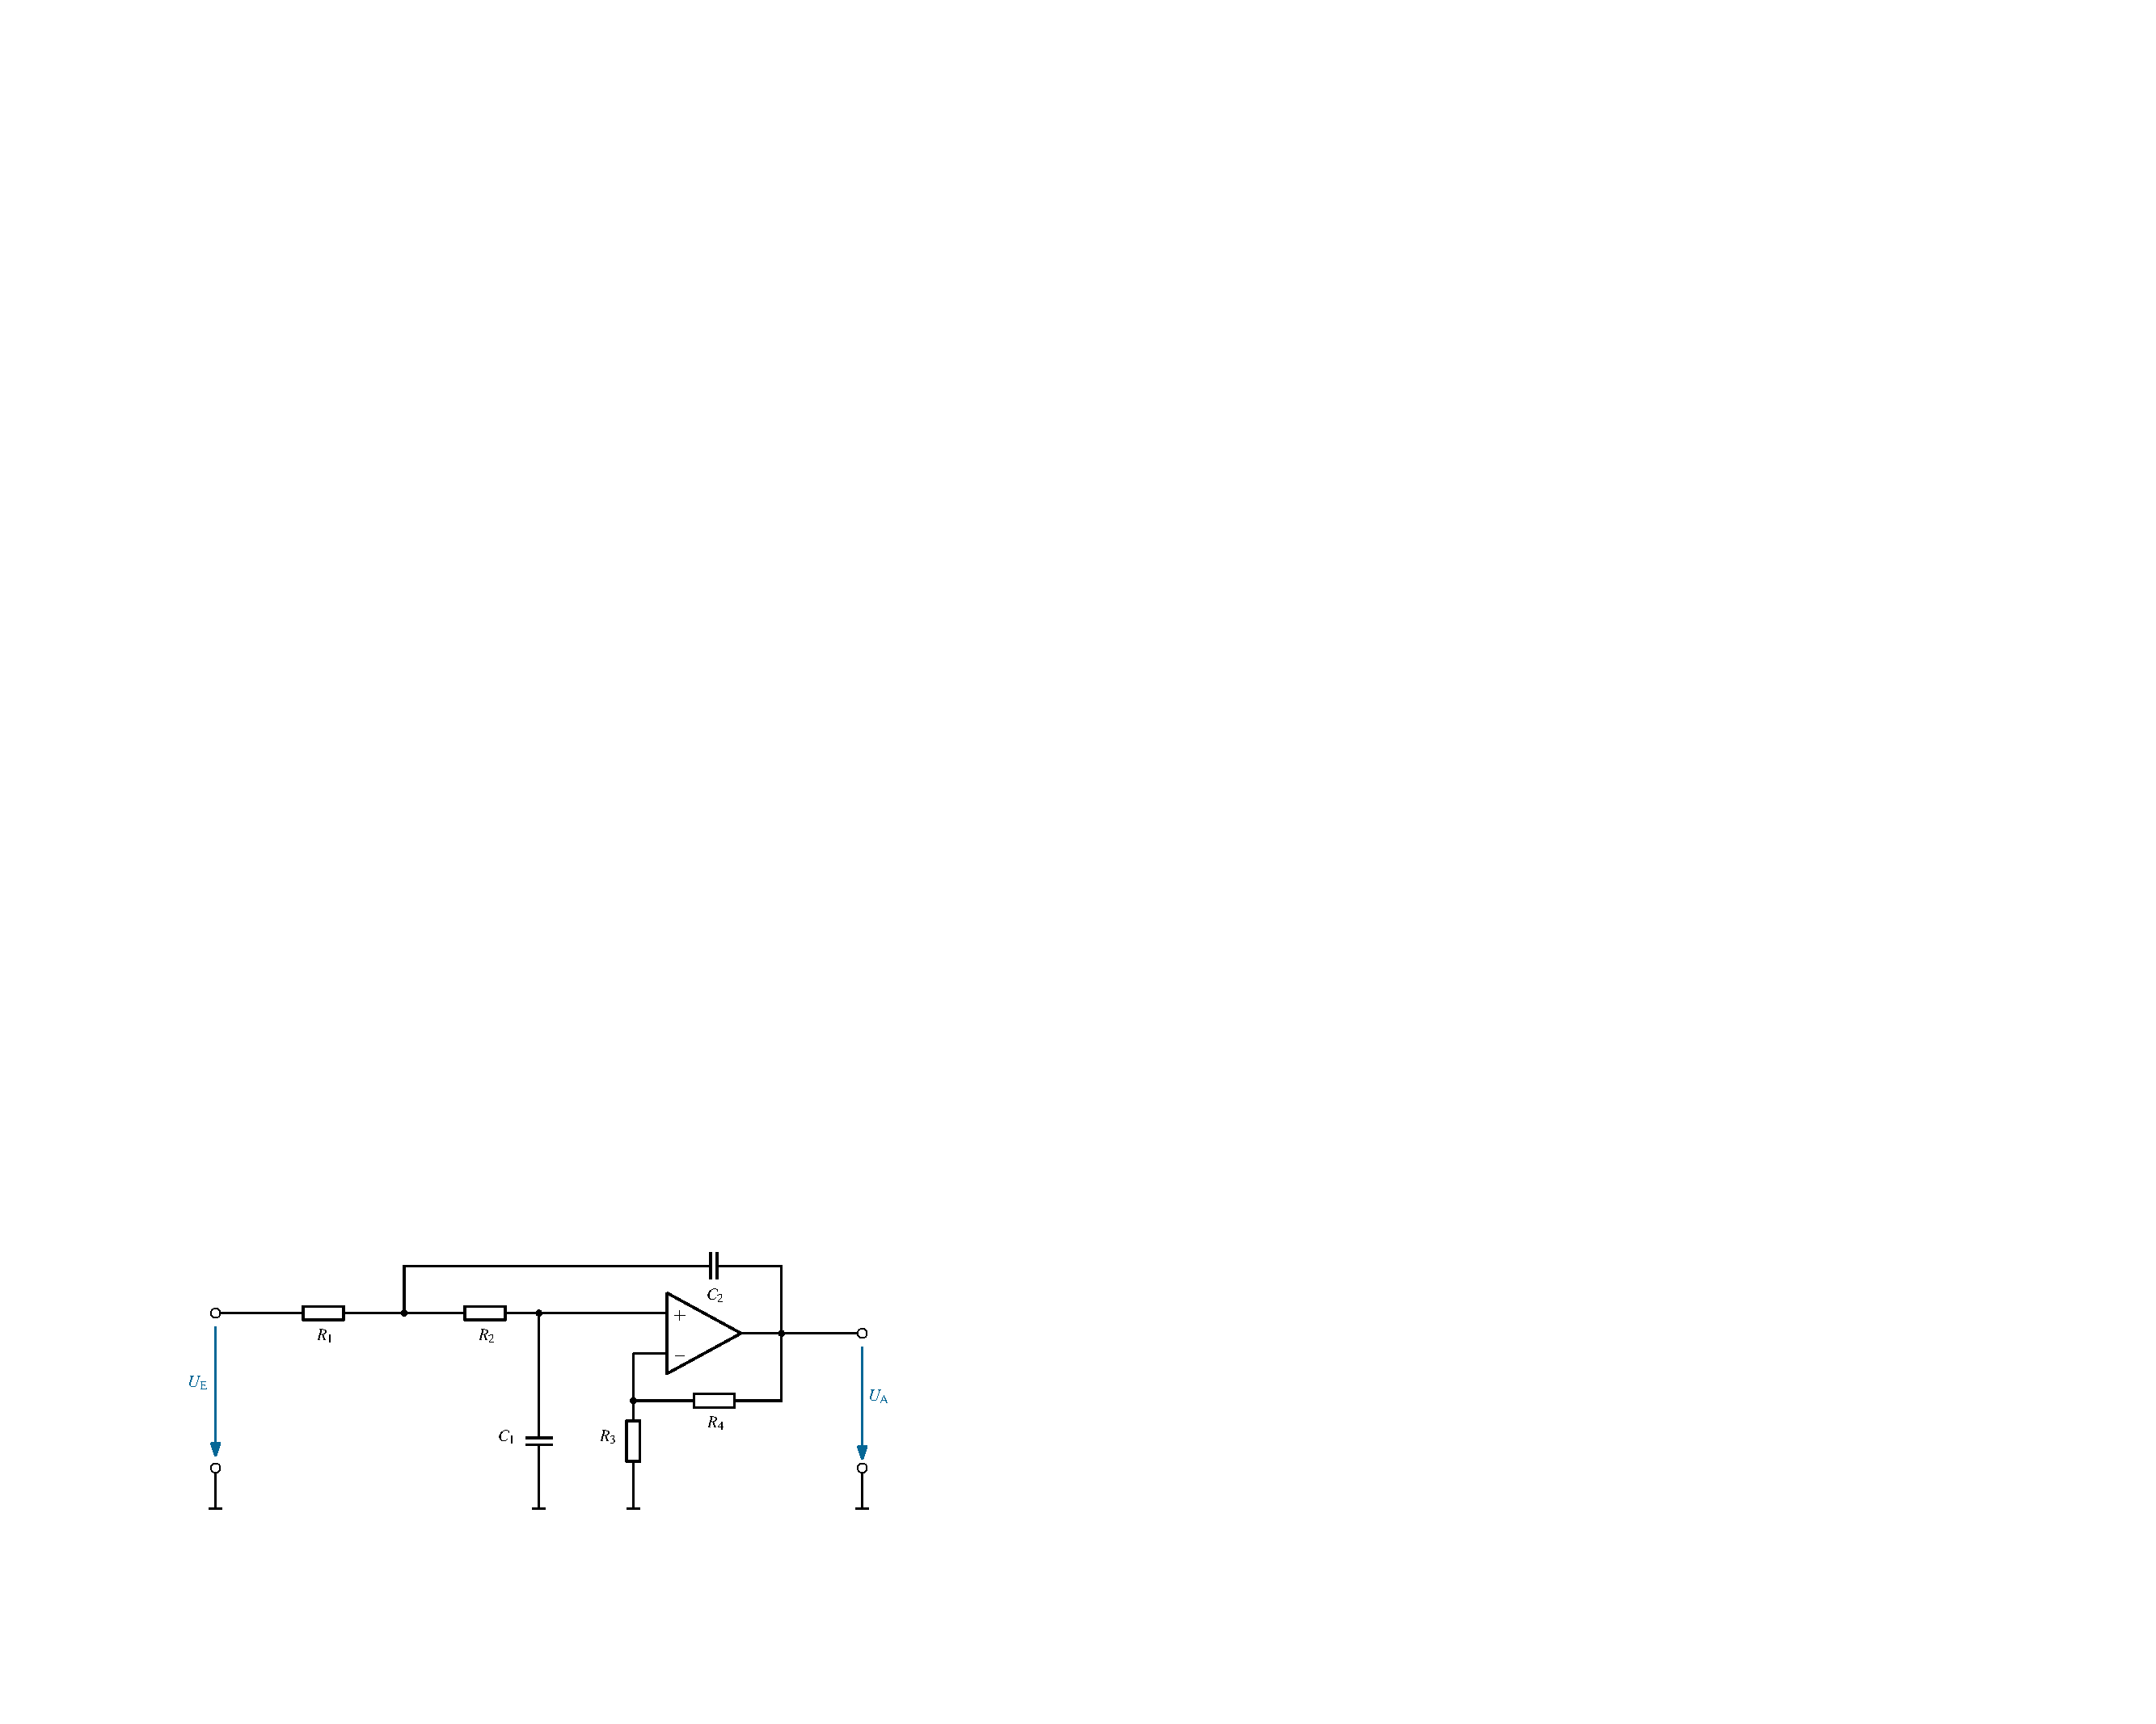
\includegraphics[scale=1]{schaltbild}
  \end{center}
\end{lstlisting}

\begin{center}
  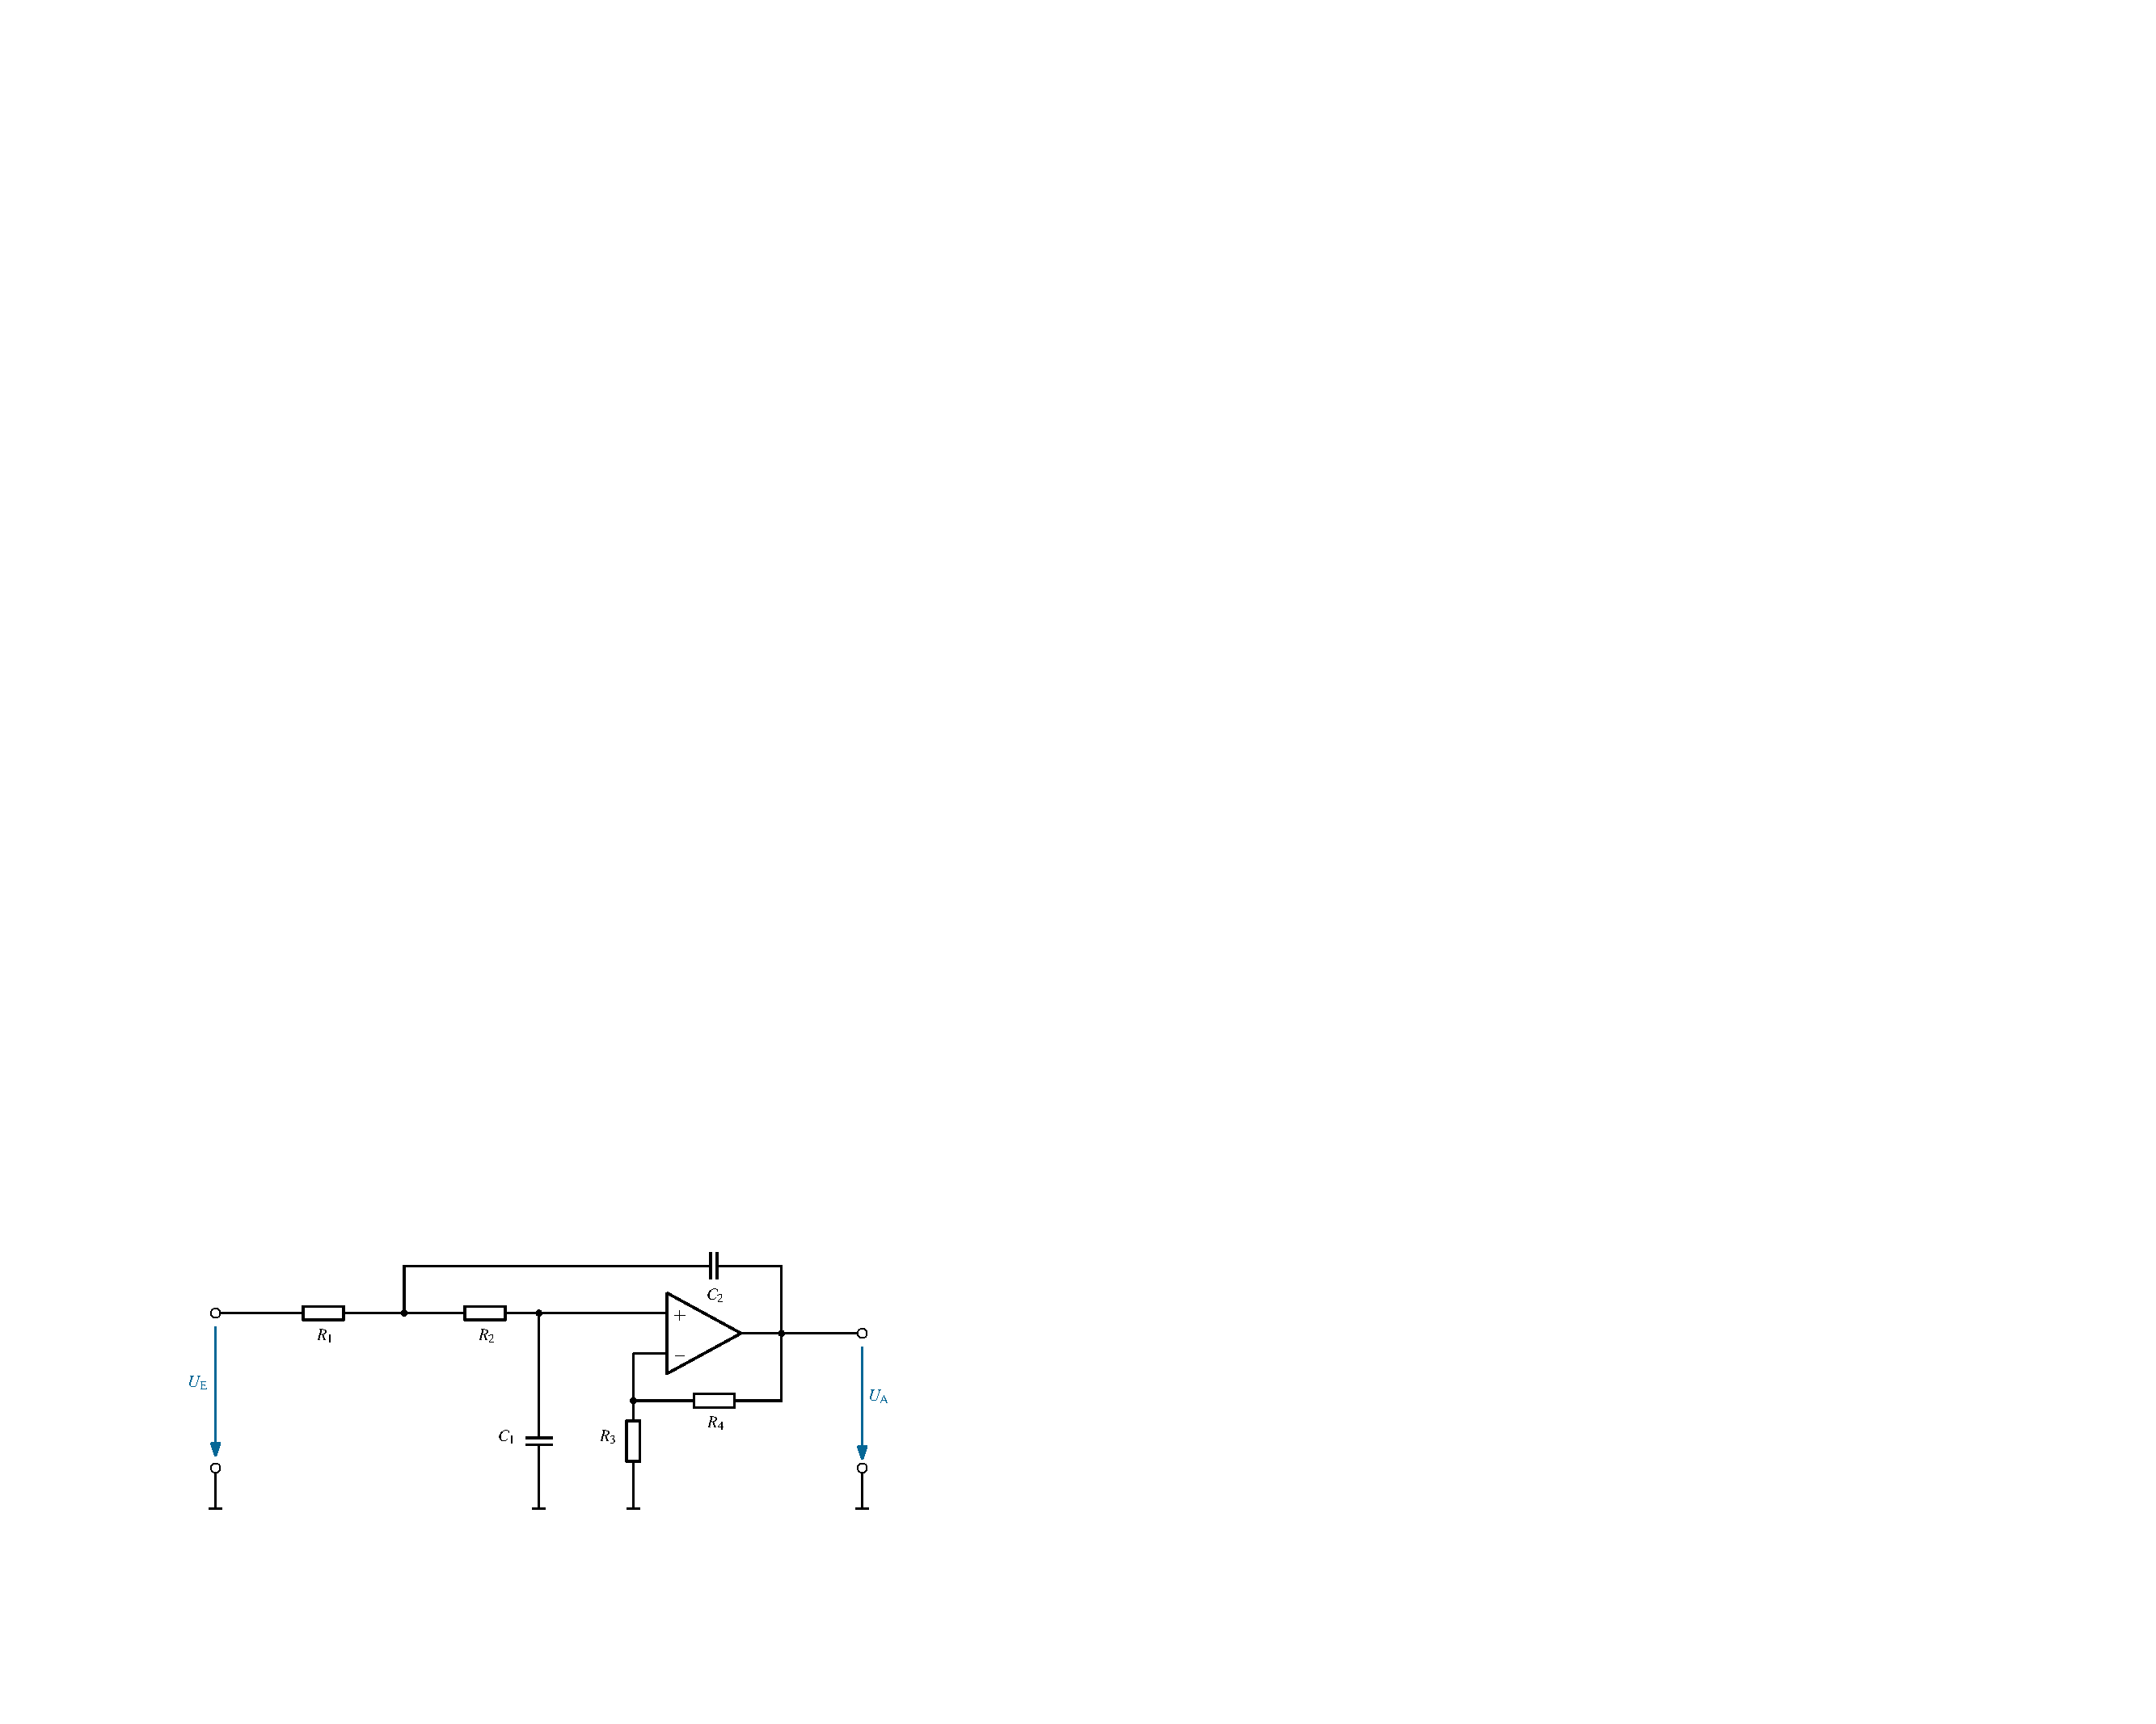
\includegraphics[scale=1]{schaltbild}
\end{center}

Es ist auch möglich, Abbildungen durch den Text \emph{fliessen} zu
lassen. \LaTeX\ kümmert sich um die Positionierung. Das Bild
\ref{fig.Filterschaltung} im Kapitel
\ref{ch.test} wird mit dem Folgenden code erzeugt:

\begin{lstlisting}
\begin{figure}[bht]
  \begin{center}
    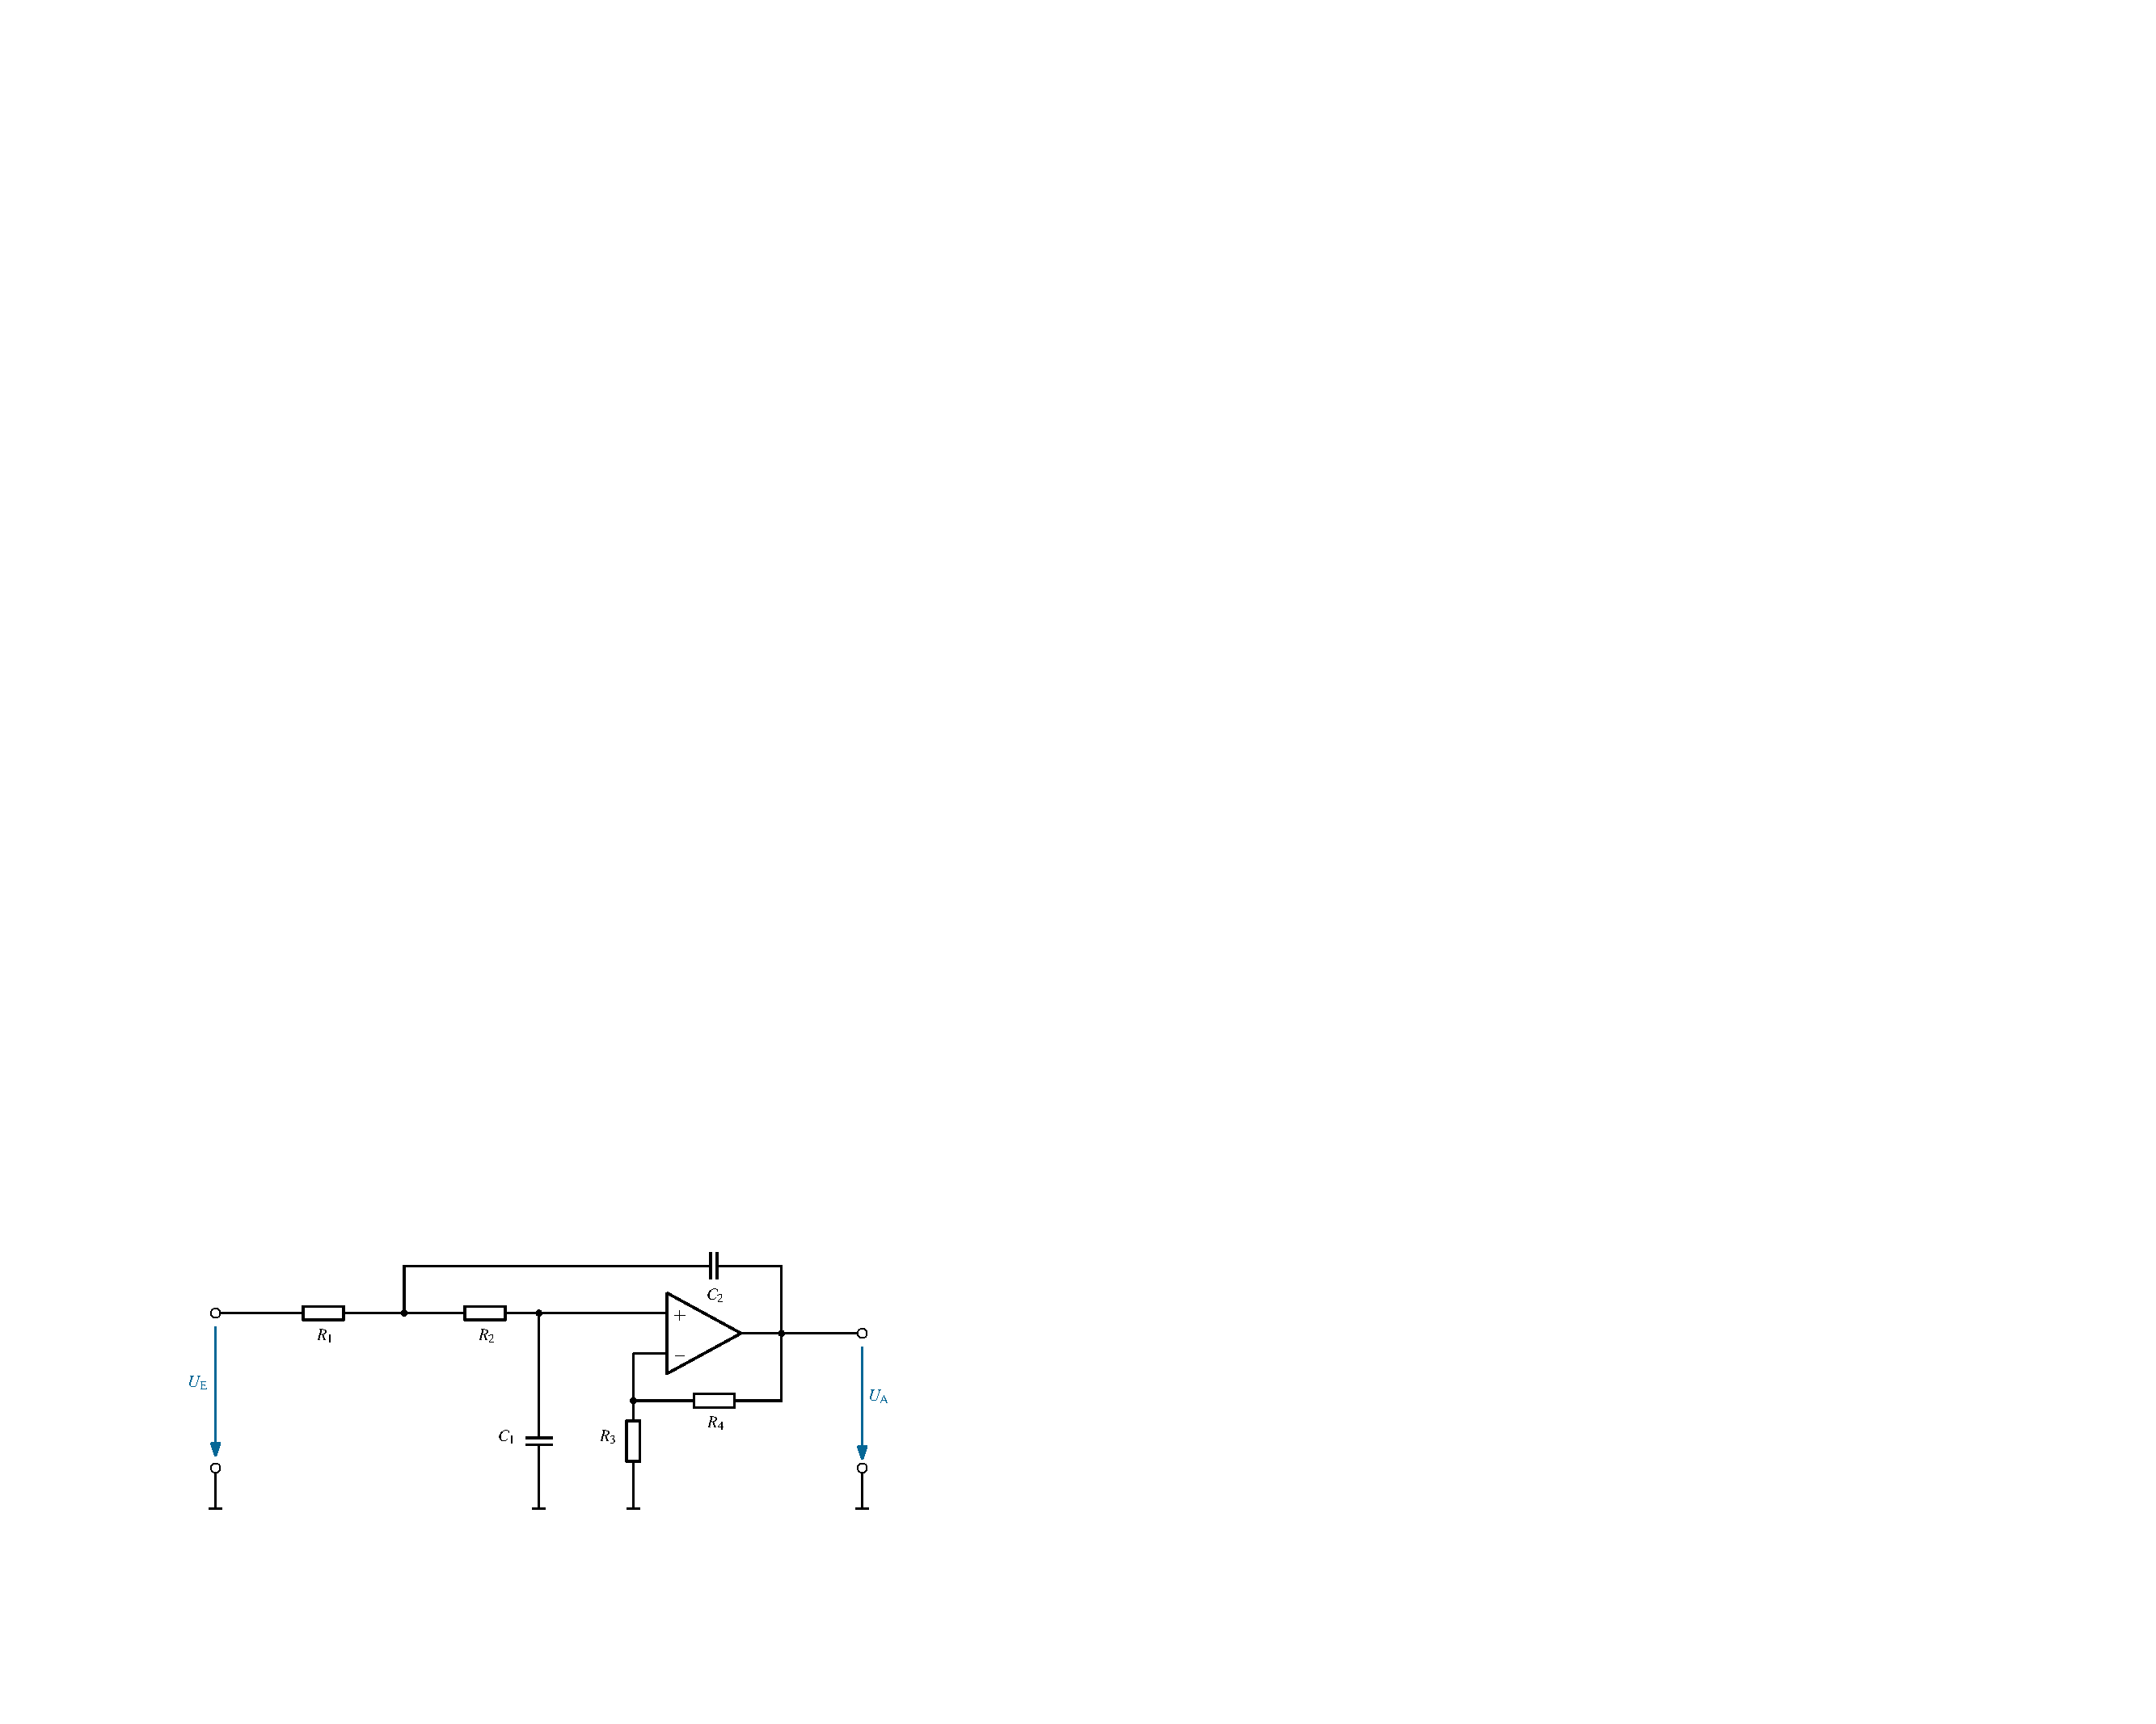
\includegraphics[scale=1]{schaltbild}
    \caption{Die verwendete Filterschaltung}
    \label{fig.Filterschaltung}
  \end{center}
\end{figure}
\end{lstlisting}

Hier ist zu  beachten, dass das Bild auch  automatisch in das Abbildungsverzeichnis
übernommen  wird.  Eine  Referenz  geschieht mit  \verb|\ref{fig.Filterschaltung}|.
Weiterhin braucht  \LaTeX\ etwas Text,  um Bilder darin \emph{fliessen}  zu lassen.
Jegliche Feinabstimmung sollte am Ende nach dem Schreiben des Textes passieren.


\section{Nützliches}

Der Textsatz kann durch viele Pakete in seiner Funktionalität erweitert
werden. Einige seien hier angeführt.

\paragraph{Transfomationssymbole}
Das Paket \texttt{trsym} definiert die Transformationssymbole fu Laplace- und
Fouriertransformation, wie Sie in einigen Lehrbüchern üblich sind.
\begin{equation}
  f(t)\,\TransformHoriz\,F(j\omega)
\end{equation} 
Viele   weitere  Symbole   und   deren  Möglichkeit   zur   Einbindung  werden   in
\cite{latex.symbols} beschrieben.

\paragraph{Querverweise anzeigen}
Das Paket \texttt{showkeys} zeigt alle  in Querverweisen verwendeten Marken im Text
an, so dass Fehler schneller gefunden werden können. 


%% \begin{bytefield}[boxformatting={\centering\itshape},
%%                   bitwidth=1.5em]{20}
%%   \bitheader[b]{0-19}   \\
%%   \bitbox{1}{\tiny F/E} & 
%%   \bitbox{1}{\tiny T0}  & 
%%   \bitbox{1}{\tiny T1}  & 
%%   \bitbox{1}{\tiny Fwd} & 
%%   \bitbox{16}{Data value} \\
%% \end{bytefield}

\chapter{Einleitung}

\anno{ca. 5 Seiten}

\begin{neu}
lässt sich hier eine Einleitung aus den Papers ableiten? ggf. Master Expose mit hinzuziehen!
  
\end{neu}
Jährlich erscheint mit den OWASP Top Ten \cite{owasptopten}  eine Liste der meist genutzten und bekannten Sicherheitsrisiken für Webanwendungen. In den meisten Fällen wird eine Anwendung sehr indiviuell gegen solche Risiken abgesichert und häufig wird dabei auch jedes einzelne Risiko separat adressiert. WebApplicationFirewalls (WAF) bieten einen relativ einfachen Weg einen Großteil der Risiken allgemein auszuschließen. Die Konfiguration einer WebApplicationFirewall muß jedoch auf die jeweilig zu schützende Anwendung angepasst werden. Mit dieser Masterarbeit soll eine Möglichkeit zur einfacheren Einbindung dieser Schutzmaßnahme bereitgestellt werden. Es wird gezeigt wie eine ältere WAF-Software auf einen neuen Stand gebracht wird und mehrere Instanzen dieser Software gekoppelt werden können. Mittels selbständiger Kategorisierung wird dem Nutzer die individuelle Konfiguration abgenommen und ein messbarer Gewinn an Sicherheit für viele Anwendungen bereitgestellt. \anno{aus Exposee übernommen}

% das grosse Problem
%% Was ist der Markt
%%% zahlreiche Anbieter teils spezialisiert auf bestimmte Bereiche; zahlreiche Arten von WAF
%% Wem hilft es?
%% Warum jetzt?
%% Ist das Problem lösbarer geworden?

\subsection{Zielsetzung}
% Ziel der Arbeit
%% Was ist Ihr relevantes Teilproblem? Was ist die zentrale Frage?
%% Ihr Ziel in zwei Absätzen.
%%% Warum genau dieses Problem?
%%% Ist Ihr Beitrag völlig neu, oder nur ein Baustein?
%%% Ist Ihr Proble schwer zu lösen oder straight forward?
%%% Eher Forschung oder Anwendung?
%%% Was machen Sie nicht? Und warum haben Sie sich entschieden das nicht zu machen.
%% Wenn Sie ein System bauen...
%%% Welche Anfragen/Aufgaben wollen Sie beantworten/lösen können?
%%% Welche Kernfunktionalität soll Ihr System haben?
%%% Was ist ein typischer (Bedienungs-)Prozess für Ihr System



% Methodik (1 Seite)
%% Wie wollen Sie das Problem lösen?
%% Welche Grundlagen müssen Sie beachten?
%% Wie ist Ihre Vorgehensweise?

% Gliederung und Aufbau (ca. 0,5 Seiten)
%% Wann lesen wir was und warum?
\subsection{Aufbau der Arbeit}

% erster Teile Grundbegriffe, verwandte Vorarbeiten und

Dieses \textbf{erste Kapitel} der Arbeit lieferte bereits einen kurzen Einblick in die Thematik. Das folgendende \textbf{zweite Kapitel} erläutert noch wichtige Grundbegriffe aus den Bereichen der IT-Sicherheit. Es folgt ein Kapitel mit Erläuterung um den eigentlichen Inhalt. \textbf{Kapitel 4} gibt einen kurzen Einblick über Arbeiten in der technischen Umsetzung. Im anschließenden Kaptitel findet in einer kurzen Demonstration die Auswertung statt und die Arbeit schließt mit einem kurzen Ausblick ab.

%Grundlagen und verwandte Arbeiten (Bitte nicht mehr als 8 Seiten)
%  Grundbegriffe
%  Thema 1
%  Thema 2 (optional)
%  Thema 3 (optional)
%  Zusammenfassung (ca. 0,5 Seiten)
%%%
%% Berliner Hochschule für Technik --  Abschlussarbeit
%%
%% Kapitel 2
%%
%%

\chapter{Zweiter Abschnitt}\label{ch.test}

In diesem Abschnitt folgt reichlich Blindtext, um das Aussehen voller Seiten zu
dokumentieren. 

\section{Grundlegendes}

\begin{neu}
  \blindtext \anno{Sachen gibt's!}
\end{neu}
\blindtext 

\section{Weiterführendes} 

\begin{neu}
  \blindtext
\end{neu}

\blindtext
\blindenumerate
\blindtext[3] \anno{Lesen, bitte!}

\begin{figure}[bht]
  \begin{center}
    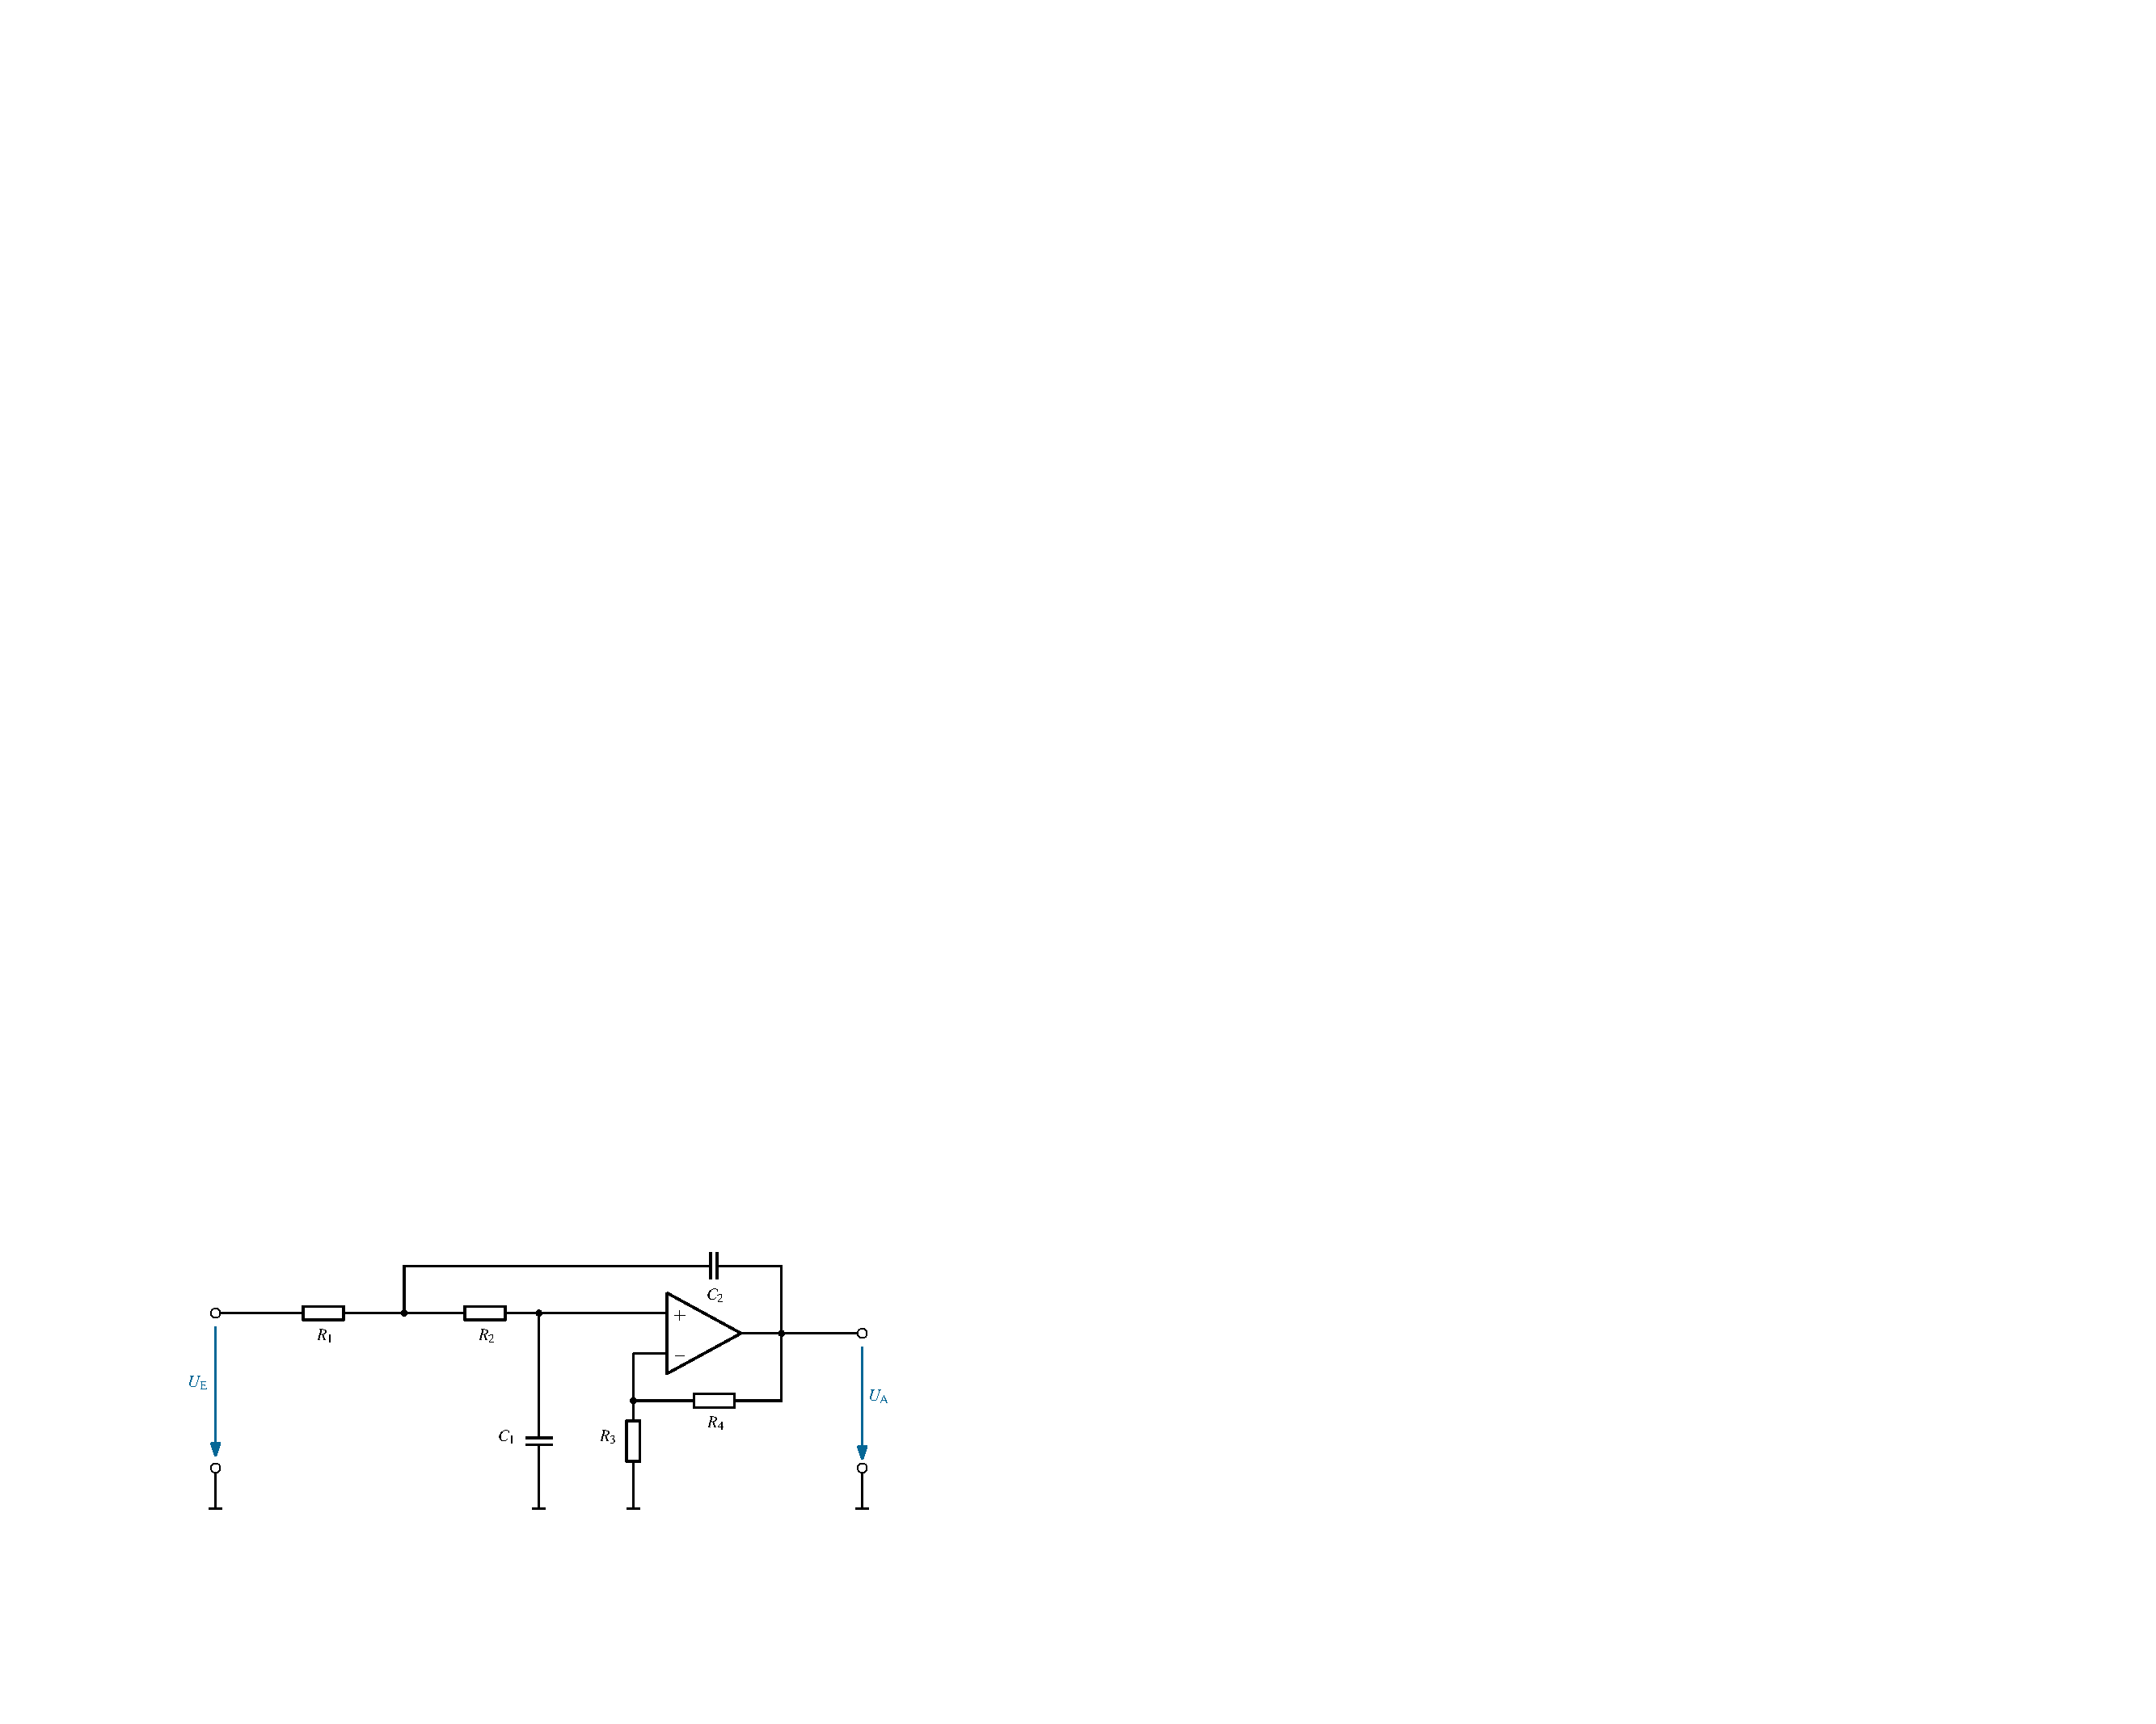
\includegraphics[scale=1]{schaltbild}
    \caption{Die verwendete Filterschaltung}
    \label{fig.Filterschaltung}
  \end{center}
\end{figure}

\blinditemize[8]
\Blindtext[2][2]
\blinddescription \anno{Es ist auch möglich längere Randnotizen zu machen. Ob die 
  dann aber gelesen werden, ist so eine Sache}  

\section{Abwegiges}

\blindtext


\chapter{Grundlagen}

\anno{bitte nicht mehr als 8 Seiten}

% Grundbegriffe 2 Seiten
\section{Grundbegriffe}
\subsection{WAF allgemein}
Um die Sicherheit einer Anwendung zu gewährleisten sind viele verschiedene Schritte notwendig, so sollten natürlich bereits in der Anwendung selbst Ein- und Ausgabemöglichkeiten, z.B. durch Validierung, Encoding, usw. überprüft und gegebenenfalls eingeschränkt werden. Dabei lässt sich nicht jeder mögliche Angriffsfall vorhersehen oder eine eigene Implementierung ist zu aufwendig und teuer, weil häufig nicht ausreichend personelle Ressourcen oder Bugdet vorhanden sind um eine Web Applikation auf alle möglichen Sicherheitslücken zu prüfen. Im Laufe des Betriebes einer Web Anwendungen können zudem neue Angriffsvarianten entstehen und zusätzlich ist gerade bei Web Applikationen der Zeitdruck zur Veröffentlichung einer solchen häufig sehr hoch.

An diesem Punkt kommen sogenannte Web Application Firewalls ins Spiel. Im Gegensatz zu regulären Firewalls haben Web Application Firewalls direkten Zugriff auf die HTTP-Anfragen (requests) und Antworten (responses) und können diese entsprechend bewerten und gegenbenenfalls blockieren oder gefährdende Inhalte filtern oder umschreiben.

%% 
\textcolor{bhtGray}{\ding{110} Definition\footnote{\url{https://owasp.org/www-community/Web_Application_Firewall} abgerufen am 30.05.2023}} A web application firewall is an application firewall for HTTP applications. It applies a set of rules to an HTTP conversation. Generally, these rules cover common attacks such as Cross-site Scripting (XSS) and SQL Injection. While proxies protect generally protect clients, WAFs protect servers. A WAF is deployed to protect a specific web application or set of web applications. A WAF can be considered a reverse proxy. WAFs may come in the form of an appliance, server plugin, or filter, and may be customized to an application to an application. The effort to perorm this customization can be significant and needs to be maintained as the application is modified.

%%
asd



\subsubsection{Anwendungsfälle}
%% Anwendungsfaelle WAF (gut beschrieben bei WAFEC2)
%% irgendwie Uebergang zu ML und WAF mit ML schaffen
%% Sammlung; payload,fuzzer,fingerprinting, bypassing

\subsection{Arten}

\subsubsection{Unterscheidung nach Position}
Grundsätzlich lassen sich solche Systeme nach ihrer Position in der Netzwerk- und Servertopologie unterscheiden. Es existieren einerseits Systeme die vor eine Anwendung geschaltet werden und Systeme die direkt in die Anwendung integriert werden. Die erste Gruppe lässt noch eine Verzweigung in weitere Unterarten, wie \emph{Reverse Proxy}, \emph{Appliance}, \emph{Plugins} für WebServer oder \emph{Passive Devices} (IDS), zu.


\subsubsection{Unterscheidung nach Abwehrmaßnahmen}

\paragraph{Regelbasierte Systeme}
Der Großteil bekannter WebApplicationFirewalls arbeitet jedoch \emph{regelbasiert}. In diesem Fall werden ein- und ausgehende Datenströme (Requests/Responses) unabhängig voneinander (zustandslos) betrachtet und einer Mustererkennung unterworfen. Häufig sind die Regeln anhand sogenannter \emph{Regular Expressions} definiert.

\paragraph{Logische Systeme}
Bei logikbasierten Abwehrmaßnahmen handelt es sich um Abwehrmaßnahmen die aufgrund von bekannten (logischen) Rückschlüssen eingeleitet werden. Einfachstes Beispiel wäre das temporäre Sperren der Loginseite bei dreimalig falschem Login. Bei Nutzung einer WAF die keine logikbasierten Auswertungen ermöglicht, müssten entsprechende Anwendungsfälle in der Anwendung selbst implementiert werden. (Oder im Fall der gerade beschriebenen Authentifizierungproblematik in einen externen Dienst ausgelagert werden.)

\subsection{Grundbegriffe allgemein}

\textbf{Bypassing:}

\textbf{Filter:}

\textbf{Fingerprinting:} Ähnlich der Abnahme und Identifizierung von Personen mit Hilfe eines individuellen Fingerabdrucks können auch Produkte wie Software anhand spezifischer Merkmale identifiziert werden. Beim \emph{Fingerprinting}

\textbf{Fuzzer:}

\textbf{Payload:}

\textbf{Regulärer Ausdruck:} Eine Zeichenkette zur Beschreibung einer Menge von Zeichenketten mit Hilfe einer vordefinierten Syntax. Ein regulärer Ausdruck kann bespielsweise genutzt werden um bestimmte Muster in einem Text zu erkennen oder einen Text mit einem Muster zu vergleichen.

\textbf{Request:} 

\textbf{Response:}

\section{Related Work} %umbenennen ca. 6

% Thema 1
\subsection{Evolution der Firewalls}

\subsubsection{Strikt nach Regeln}

Die praktisch einfachste Web Application Firewall wäre \emph{-beispielsweise-} eine einfache Regel innerhalb der Webserver-Konfiguration, die anhand eines bestimmten Merkmals den Datenverkehr entweder korrekt beantwortet oder \glqq\emph{abwehrt}\grqq. Wenn nicht explizit entnommen findet sich der folgende Eintrag in jeder Konfiguration des \emph{Apache httpd}-Servers und sorgt dafür dass der Zugriff auf jede Datei deren Dateiname mit \texttt{.ht} beginnt unterbunden wird:

\lstset{language=XML,
 	basicstyle=\ttfamily\color{black}\small,
 	keywordstyle=\bfseries\color{bhtBlue},
 	identifierstyle=\color{black}, 
 	commentstyle=\color{gray}\textsl
      }
%      \begin{figure}
%        \caption{Beispiel für einfache Regel}
%        \label{fig:httprule}
\begin{lstlisting}
  <Files ".ht*">
    Require all denied
  </Files>
\end{lstlisting}
%      \end{figure}

Mit steigender Komplexität der zu schützenden Anwendungen steigt auch der Bedarf an Regeln. Zu berücksichtigende Auswahlkriterien beschränken sich dann auch nicht nur auf den \glqq\emph{Dateinamen}\grqq. Attribute wie der Aufrufzeitpunkt, der Inhalt des Aufrufs, die Identität des Aufrufenden und viele andere Kriterien können zu entscheidenden Faktoren werden. Im Sinne der Entkopplung wurde diese Filterlogik häufig in entsprechende Module oder Plugins ausgelagert. Aufgrund des hohen Verbreitungsgrades des \emph{Apache httpd}-Servers wurde dessen \emph{modSecurity}-Modul zu einem der bekanntesten Vertreter einer Web Application Firewall. Dabei handelt es sich um eine frei verfügbare und als \emph{Open Source} entwickelte Softwarelösung, die eine eigene Sprache zum Erstellen der WAF-Regeln mit sich bringt. Der obige Aufruf zum Verhindern des Zugriffs auf Dateien die mit \texttt{.ht} beginnen lautet:

\lstset{language=bash,
 	basicstyle=\ttfamily\color{black}\small,
 	keywordstyle=\bfseries\color{bhtBlue},
 	identifierstyle=\color{black}, 
 	commentstyle=\color{gray}\textsl
      }
\begin{lstlisting}
  #SYNTAX: SecRule VARIABLES OPERATOR [ACTIONS]        
  SecRule REQUEST_URI ".ht*" "deny"
\end{lstlisting}
% end figure

Bei dieser Sicherheitsregel \verb=SecRule= wird die aufgerufene Adresse \verb=VARIABLES= auf Übereinstimmung mit einem regulären Ausdruck \verb=OPERATOR= geprüft und bei Übereinstimmung die Ausführung verweigert \verb=ACTIONS=.

\subsubsection{Allgemeine Regeln}
Mit der Zeit entwickelten sich immer mehr und immer komplexere Regeln. Regeln wurden auf spezielle Anwendungen, Anwendungsfälle oder Angriffsszenarien zugeschnitten und gesammelt. Es entstanden Sammlungen die unter Administratoren, Entwicklern und anderen IT-Spezialisten ausgetauscht wurden.
Im Oktober 2006 veröffentlichte das \emph{Open Web Application Security Project} erstmals eine allgemein verfügbare Sammlung von generischen Regeln für das modSecurity-Modul mit dem Ziel ein Art Grundschutz zur Absicherung von Webanwendungen anzubieten. Die als \emph{OWASP Core Rule Set} bekannte Sammlung wird seitdem stetig erweitert und weiter entwickelt. Wirft man heute einen Blick in die verfügbaren Regeldateien des Projekts \footnote{\url{https://github.com/coreruleset/coreruleset/tree/v4.0/dev/rules} abgerufen am 01.06.2023} findet man sowohl allgemeine Regeln mit Bezug auf die Angriffsmuster aus den OWASP Top10 \cite{owasp10}, als auch Regeln die sehr speziell auf bestimmte Anwendungen oder Sicherheitsvorfälle ausgelegt sind.

Obwohl die bereitgestellten Regeln des Core Rule Sets eine gewisse Basissicherheit bieten können, sind diese nur als Ausgangsbasis zur (produktiven) Absicherung von Anwendungen zu sehen. Erstens wird nicht jeder Fall berücksichtigt und zweitens erzeugen die Regeln unter Umständen auch Fehlmeldungen (Falsch-Positive). 

% einfache regel => firewall
% Systeme zum verwalten der Regeln
% Standardisierte Regeln (OWASP CRS)

\subsubsection{Hybride Ansätze}

% Krueger Manaseer etc.

\subsubsection{Fortschritte in Richtung Intelligenz}

Collaborative Detection \cite{karakannas2014}

% kruegel gimenez appelt kozik testen mit ML Ansätzen

% Thema 2
\subsection{Thema 2 - ML}

%ansaetze und kombination?

% Thema 3 optional die andere seite
\subsection{hacking Wafs}


% Zusammenfassung (ca. 0,5 Seiten)
\section{Zusammenfassung}

% ggf. ditaa tabelle ueber den Zeitverlauf der verschiedenen Arbeiten nach Attack-Defend-Muster


November 2002 modSecurity 1st release
Oktober 2006 OWASP CRS
August 2009 CRS 2
2014 Collaborative Detection
2016 CRS3.0.0 CRS Sampling Mode

%Kern der Arbeit (ca. 15 - 20 Seiten)
%  Probleme und die Lösungsansätze
%  Methodik/Vorgehen (diesmal ausfuehrlich)
%  Uebersicht bzw. Architektur
%  Oder aber: Der xxx Algorithmus
%  Optional: Der yyyy Algorithmus
%  Zusammenfassung (ca. 0,5 Seiten)
te\chapter{Kern der Arbeit}

\anno{ca. 15-20 Seiten}

% Probleme und die Loesungsansaetze
\section{Probleme}

Der im vorherigen Kapitel betrachtete zeitliche Rahmen, über die Entwicklung von Web Application Firewalls, umfasst mehr als zwanzig Jahre. Ein Zeitraum in dem sich zahlreiche Produkte in diesem Bereich etablierten. Im Anhang finden Sie, beispielsweise, unter \ref{tab:my_wafwoof} eine (nicht vollständige) Liste von derzeitigen WAF-Produkten verschiedener Hersteller. Über den gesamten Zeitraum haben sich Webtechnologien weiterentwickelt und auch die Art und Weise der Nutzungs des Internets änderte sich. Mit der Verbreitung der Smartphones und Sprachassistenten wurden aus einfachen Webangeboten vielschichtige Anwendungen mit verschiedenen möglichen Clientsystemen (\emph{mobile-first-Ansatz}). Serviceorientierte Architekturen, Webservices, Microservices, Künstliche Intelligenz - alles entwickelte sich weiter. Im Bereich der IT-Sicherheit veröffentlichte das \emph{Open Web Application Security Project} 2019 erstmals eine Liste seiner zehn kritischsten Sicherheitsrisiken explizit für den Bereich der \emph{API}s. \emph{ModSecurity} ist immernoch der defacto-Standart für regelbasierte WAFs und praktisch so gut wie der einzige verbliebene Vertreter der Web Application Firewalls aus dem OpenSource-Bereich. Freie anomaliebasierte Systeme sind so gut wie nicht existent und die privatwirtschaftlichen Akteure lassen sich kaum in die Karten schauen. \\
Mittlerweile sind bereits dreizehn Jahre seit dem Erscheinen des Datensatzes CSIC2010 vergangen und schaut man in die derzeitig vorhandene Literatur scheint auch kein Nachfolger in Sicht. \\\\

\textcolor{bhtGray}{\ding{110} Applebaum über den Datensatz CSIC2010~\cite{Applebaum2021}} Gimenéz et al. provide an HTTP dataset intended to be used for the development and testing of Intrusion Detections Systems and WAFs. ... The dataset has been used extensively by other researchers ... There is still a need for a development of a new dataset as previous datasets had become outdated and did not target real systems. The dataset .. is itself now over 10 years old and targets a bespoke e-commerce system. \\\\


%

\subsection{Aufbau des Datensatzes CSIC2010}

% Aufbau /motivation von gimenez

% Aufbau
Der Datensatz besteht aus drei Teildatensätzen. Der erste Teildatensatz ist dabei für die Trainingsphase gedacht und enthält nur den normalen Datenverkehr. Die anderen beiden Teildatensätze sind für die Testphase gedacht, ein Teildatensatz mit normalem Datenverkehr und ein Teildatensatz mit \emph{bösartigem} Daten (siehe \cite{csic2010}). Die einzelnen Dateneinträge der drei Teildatensätze sind gleich aufgebaut und beinhalten



\subsection{Alter des Datensatzes}

\subsubsection{Das HTTP-Protokoll}

%% Erweiterung HTTP
\subsubsection{Neue Anwendungsarchitekturen}
%% Änderungen Anwendungsarchitekturen

\subsection{Ziel des Datensatzes}

Erhöhung der allgemeinen Gültigkeit (Diskrepanz mit spezieller Zuschneidung auf Anwendung)
Erhöhung der Genauigkeit

% SChönes Beispiel für Fortschritt, produktiven Einsatz und zeitliche Veränderung und wo Gimenez nicht funktioniert-- > PUT als anomalie in CSIC2010 definiert aber in REST durchaus üblich
% rest beispiel mit PUT

%\lstset{language=XML,
% 	basicstyle=\ttfamily\color{black}\small,
% 	keywordstyle=\bfseries\color{bhtBlue},
% 	identifierstyle=\color{black}, 
% 	commentstyle=\color{gray}\textsl
%      }
      \begin{figure}
        \caption{Beispiel für einfachen REST-Request}
        \label{fig:restputexample}
      \begin{lstlisting}
PUT /user/devtty HTTP/1.1
Host: petstore.devtty.de
Content-Type: application/json

{
  "id": 2334,
  "username": devtty,
  "firstName": "Denis",
  "lastName": "Renning"
}
\end{lstlisting}
\end{figure}



% Methodik und Vorgehen
\section{Methodik}

% Uebersicht Architektur

\section{Lösungen}

\subsection{Unzureichende Kategorisierung im Datensatz}
% Problem zu viele Falsch-Positive/Zuordnung:Framework/Status(Session) -> Anwendungsstatus (DeltaspikeClientId/SpringExecuteID)
% möglichkeit anomalien nicht auf basis der Regeln sondern auf basis von abweichungen in der Anwendungsnutzung auszuwerten

% Erweiterung Datenset um Variablen (eingeloggt/framework/id)

\begin{figure}[ht]
  \begin{center}
    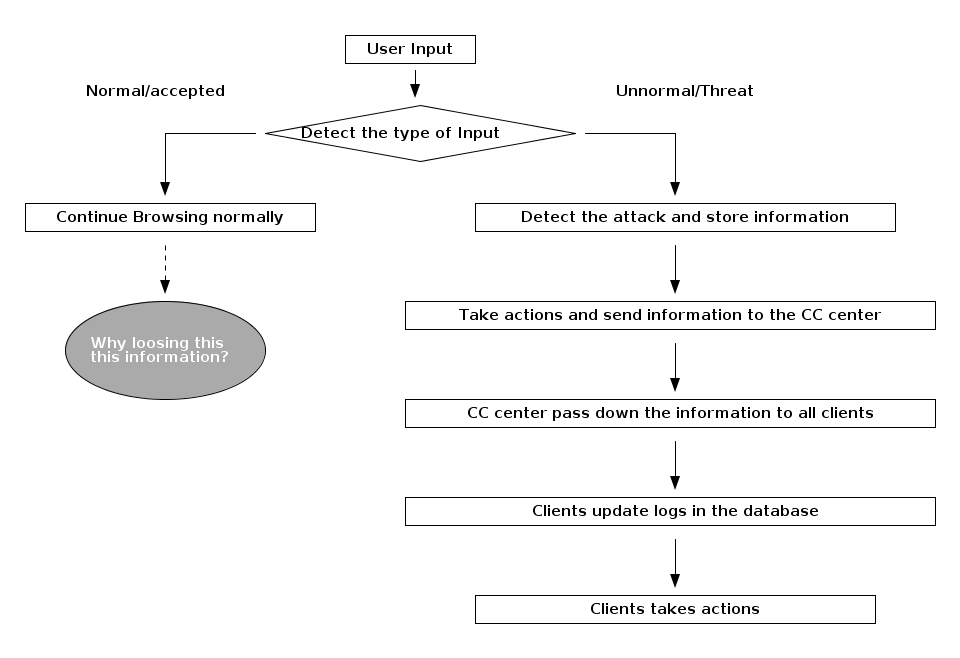
\includegraphics[width=15cm]{waf_mana}
    \caption{Zentralisiert~\cite{Manaseer2018}}
    \label{fig.topten}
  \end{center}
\end{figure}


% Oder: Der xxx Algorithmus

% Oder: Der yyy Algorithmus

% Zusammenfassung: ca. 0,5 Seiten
\section{Zusammenfassung}

\begin{neu}
  Anfang mit Aufnahme des Altenbestands, hinzufügen Entwicklungsumgebung, Test, etc

  Entwicklung Zentrale Steuerung

  Entwicklung ML Anteil
\end{neu}

%Implementierung (max. 5 Seiten)
%  Highlight 1 der Implementierung
%  Highlight 2 der Implementierung
%  Highlight des Deployments beim Kunden
%  Zusammenfassung (ca. 0,5 Seiten)
\chapter{Implementierung}

\anno{max. 5 Seiten} %Ref hat 12

% Was lesen wir in diesem Kapitel?
% Warum muss ich das als Gutachter lesen
% Wie verknüpft sich der Inhalt mit dem vorhergehenden Kapitel?
% Welche Implmentierungsentscheidungen? Welche Alternativen? Vor- und Nachteile des eigenen Ansatzes?

% Highlight 1 der Implementierung
Wie bereits in Abschnitt \ref{sec:Probleme} angemerkt sind offene Implementationen von Web Application Firewalls eher die Ausnahme und selbst Umsetzungen der in Abschnitt \ref{sec:relatedwork} erwähnten Produkte sind praktisch nicht auffindbar. In diesem Kapitel gibt es einen kurzen Überblick wie die Vorschläge aus dem vorhergehenden Kapitel dennoch praktisch umgesetzt werden können.

Eine komplette Umsetzung ohne vorherige Basis wäre zeitlich (von einer einzelnen Person) nicht umsetzbar gewesen, daher sollte ein vorhandenes Open Source Produkt entsprechend erweitert werden. Bei der Auswahl wurden zuerst die zwei (leichtgewichtigen) Lösungen \emph{OWASP ESAPIFilter}\footnote{\url{https://owasp.org/www-project-enterprise-security-api/} abgerufen am 05.07.2023} und {SpringSecurity HttpFirewall}\footnote{\url{https://docs.spring.io/spring-security/reference/servlet/exploits/firewall.html} abgerufen am 05.07.2023} betrachtet. Beide Produkte verstehen sich als Ausgangsbasis für die Entwicklung sicherheitsrelevanter HTTP-(Servlet)-Filter auf Anwendungsebene, sämtliche Funktionalität muß jedoch vom Nutzer erst implementiert werden. Bei der Nutzung wäre ein erhöhter Arbeitsaufwand absehbar. Diogo Sampaio und Jorge Bernardino verglichen 2017 verfügbare WAFs die ebenfalls als Erweiterungskandidaten in Frage kamen (siehe Tabelle \ref{tab:my_vergos}).

% Tabelle ggf. in Anhang verschieben

\begin{table}[h]
  \centering
  \begin{tabular}{|c | c | c | c |} 
    \hline
    & \textbf{ModSecurity} & \textbf{WebCastellum} & \textbf{IronBee} \\ [0.5ex] 
    \hline
    Simple filtering & Yes & Yes & Yes \\ 
    \hline
    Regular expression based filtering & Yes &  & Yes \\
    \hline
    Auditing & Yes &  & Yes \\
    \hline
    Null byte attack prevention & Yes & Yes &  \\
    \hline
    URL Encryption & Yes & Yes &  \\ [1ex] 
    \hline
    Stateful Attack Detection & & Yes & Yes \\
    \hline
  \end{tabular}
  \caption{Vergleich Open Source Web Application Firewalls (aus \cite{Sampaio2017}) }
  \label{tab:my_vergos}
\end{table}

\emph{ModSecurity} und \emph{IronBee}s Stärken liegen in der regelbasierten Auswertung (\emph{regular expression based filtering}). Beide werden als Reverse-Proxy vor der eigentlichen Anwendung eingesetzt und sind keine HTTP-Servlet-Filter. Dies hat den Nachteil das kein Zugriff auf die eigentlichen Anwendungsdaten besteht und nur anhand des HTTP-Datenverkehrs gefiltert werden kann. \emph{WebCastellum} scheint hier Gutes aus beiden Welten bereit zustellen, zum einen (als Servlet-Filter) direkten Zugriff auf die Anwendungsdaten anzubieten, als auch regelbasiertes Filtern \emph{out-of-the-box}. \anno{Achtung! Sampaios Tabelle ist hier fehlerhaft! Übernehmen trotz Fehler?}
Mit Hinsicht auf einen späteren produktiven Einsatz wurde daher die Software \emph{WebCastellum} als Grundlage für die Implementierung der Firewall-Funktionalität gewählt.

\section{Vorarbeiten}

Leider haben WebCastellum und der CSIC2010 Datensatz eine Gemeinsamkeit - das Alter. Die derzeit aktuelle offizielle Version 1.8.3 von WebCastellum erschien bereits im Jahr 2009 und eine Weiterentwicklung fand seit dem nicht statt. Dennoch befindet sich das Produkt weiter in Verwendung und wird wohl auch in neuen Anwendungen genutzt, lässt zumindest die aktuelle Downloadstatistik (siehe \ref{fig:downloadwc}) vermuten. Insgesamt wurde das Binärpaket von WebCastellum in der Version 1.8.3 seit 2009 mehr als 8500 mal heruntergeladen (Stand vom 05. Juli 2023) - nicht berücksichtigt sind alle Vorgängerversionen und die Downloads über Repository-Dienste, wie z.B. Maven Central, stattfanden.

\begin{figure}[h]
  \centering
  \begin{gnuplot}[terminal=png,scale=.7]
    set datafile separator ','
    set xdata time
    set timefmt "%Y-%m"
    set xrange ["2009-01":"2023-09"]
    set format x "%b %y"
    set key autotitle columnhead
    plot '04_Implementierung/downloads.csv' using 1:2 with boxes fs solid 1.0 fc 'steelblue'
  \end{gnuplot}
  \caption{Download-Statistik SourceForge WebCastellum 1.8.3 binary}
  \label{fig:downloadwc}
\end{figure}

Vor den eigentlichen Arbeiten waren also noch ein paar kleinere Vorarbeiten notwendig. In einem ersten Schritt wurde der Quellcode aus dem SourceForge-Repository heruntergeladen und in ein eigenes git-Repository\footnote{\url{https://github.com/devtty/webcastellum/} abgerufen am 05.07.2023} übertragen. 

\subsection{Version 1.8.4. - Review des Quellcode und IT-Sicherheit}
Während die Binär-Distribution mit der Versionsnummer 1.8.3 verteilt wird, sind die Quellen bereits mit der nächsten Minor-Version versehen. Diese lassen sich auch fast problemlos kompilieren und zu einem verwendungsfähigen Paket zusammenbauen. Das Projekt hat nur sehr wenig Abhängigkeiten zu weiteren Bibliotheken und diese (laut durchgeführtem OWASP dependency-check) keine bekannten Schwachstellen. Etwas problematisch ist die Abhängigkeit zu älteren Bibliotheken (\emph{javax.jms} und \emph{javax.mail}), da diese nicht mehr (direkt) über den Standard-Build-Mechanismus verfügbar sind, sich aber über Umwege auftreiben lassen.

Im weiteren Verlauf wurden die Quellen noch an Githubs eigenes CI/CD-System angebunden und automatisiert einer Codeanalyse auf der Sonarcloud-Plattform \footnote{\url{https://sonarcloud.io/project/overview?id=devtty_webcastellum} abgerufen am 05.07.2023} unterzogen. Insgesamt fielen dabei im Quelltext sechs direkte Schwachstellen und 58 potentielle Schwachstellen (siehe \ref{fig:my_sonar1}) auf. Bei den direkten Schwachstellen handelt es sich um:

\begin{itemize}
    \item 3 x Verwendung schwacher Kryptographie (hier AES; Cryptographic Failures / Security Misconfiguration )
    \item 2 x Ausgabe der Session-ID in Log-Dateien (Insecure Design/Broken Authentication)
    \item 1 x XML External Entity Injection Attack (Security Misconfiguration / XML External Entities (XXE))
\end{itemize}

Wobei die XXE-Attacke von Sonar als Blocker eingestuft wird. Bei den 58 Security Hotspots handelt es sich meistens um direkte Ausgaben im Fehlerfall (\verb=printStackTrace()=) mit der Bitte zur Überprüfung das diese im Produktivbetrieb nicht ausgegeben werden. 

Inklusive Code Smells bemängelte Sonar den Quellcode in insgesamt 2657 Fällen und berechnet die angehäuften technischen Schulden auf 52 Personen-Tage Nacharbeit. 

\begin{figure}
    \centering
    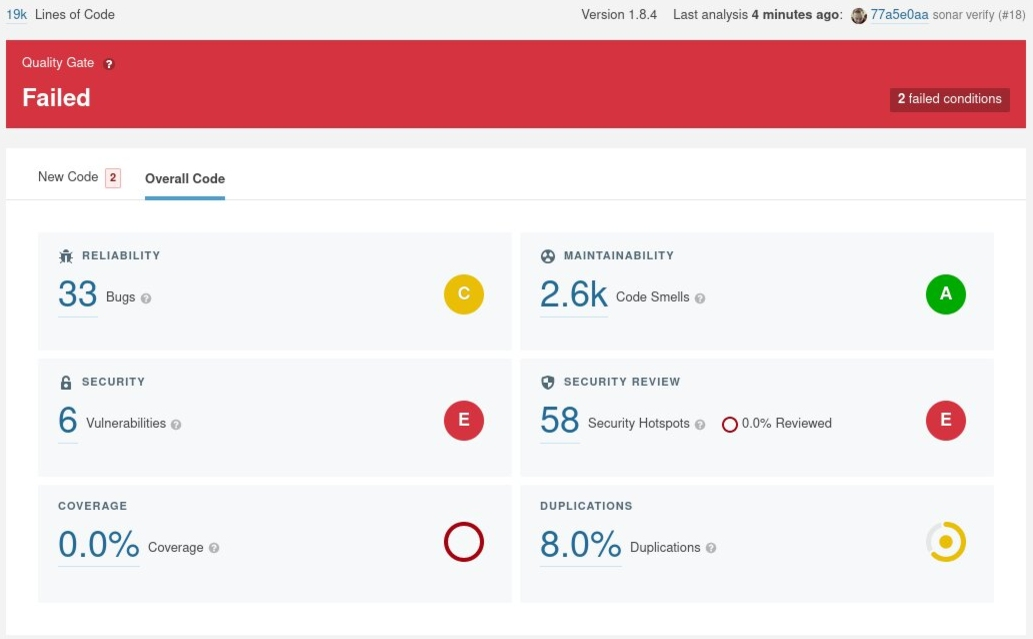
\includegraphics[width=\textwidth]{first_sonar2.jpg}
    \caption{SonarCloud erste Sichtung}
    \label{fig:my_sonar1}
\end{figure}

\begin{figure}
    \centering
    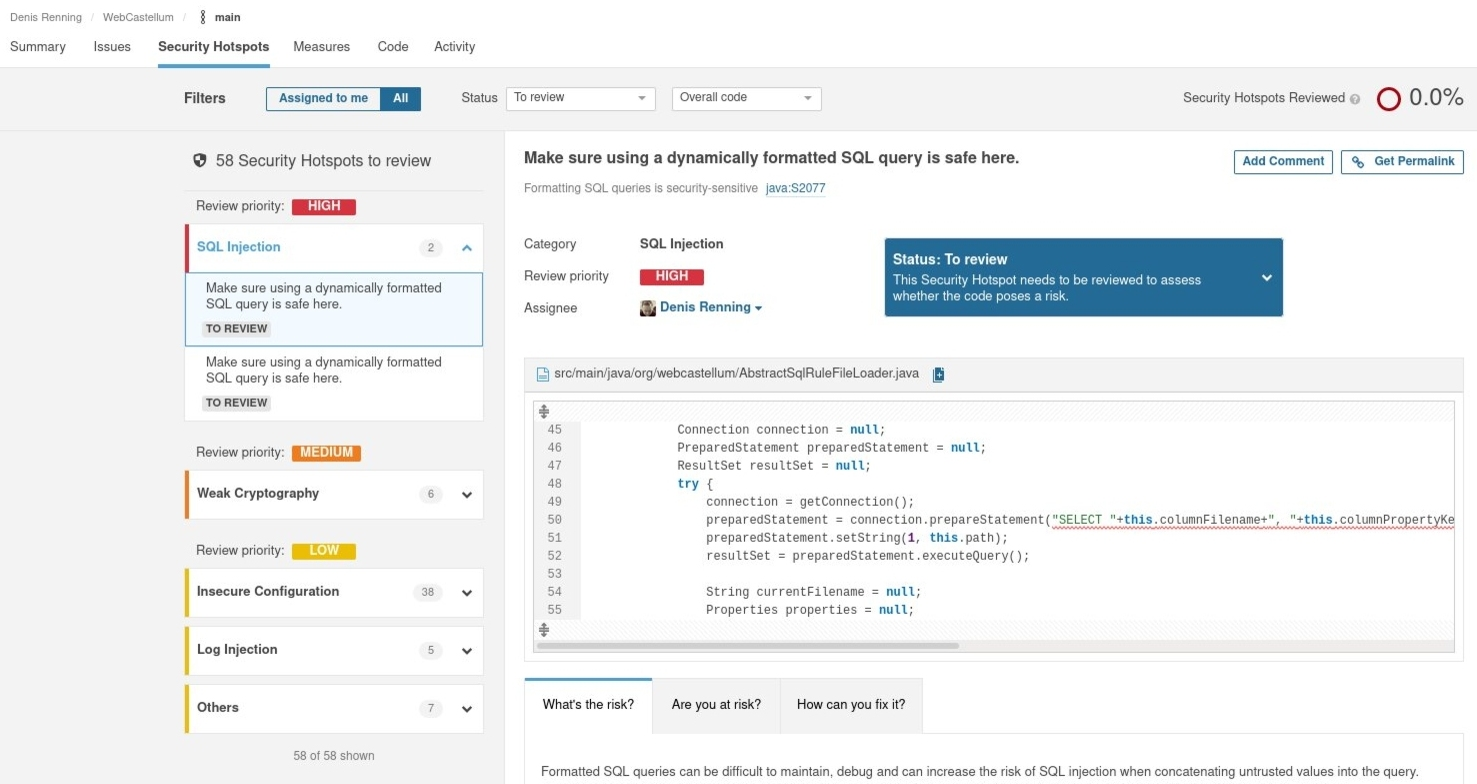
\includegraphics[width=\textwidth]{first_sonar_sql.jpg}
    \caption{SonarCloud SQL-Injection}
    \label{fig:my_sonar2}
\end{figure}



\subsection{ToDos, Unit-Tests,  etc.}

Interessant war ebenfalls die Suche nach \verb=TODO=-Markierungen im Quelltext. Insgesamt 243 mal traten entsprechende Kommentare im Quelltext auf und markierten Stellen an denen die Entwickler Probleme und Verbesserungen vermuteten bzw. Aufgaben für die nächste Version notierten. Diese Notizen reichten von einfachen Aufgabenstellungen, wie \glqq\emph{add proper logging}\grqq, über Refactoring-Ideen bis hin zu Anmerkungen deren Umsetzung die Funktionsweise des Filters beeinflussen würden. \anno{Zitierung aus eigener unveröffentlichter notwendig?}

Einige der Todo-Anmerkungen ließen auf eine geplante Überführung des Quellcodes von Java in der Version 1.4 auf Java 5 schließen. Häufig fanden sich auch auskommentierte dementsprechende Fragmente und, insbesondere bei der Verwendung listenähnlicher Objekte, fallen die in Java 5 eingeführten \emph{Generics} (s. Abbildung \ref{fig:my_l2} auf.

\begin{figure}[h]
  \begin{small}
    \begin{lstlisting}[language=java]
    // TODO: in Utility-Klasse packen (ServerUtils)
    private static void concatenateParameterMaps(
      final Map/*<String,String[]>*/ parameters, 
      final Map/*<String,String[]>*/ parameterMapToAdd) {
    \end{lstlisting}
  \end{small}
  \caption{Auszug aus WebCastellumFilter als Beispiel für ToDos und auskommentierte Generics}
  \label{fig:my_l2}
\end{figure}
  
Dabei sollte berücksichtigt werden, dass diese Kommentare aus dem Jahr 2009 stammen und auch die Programmiersprache Java in den letzten Jahren deutliche Fortschritte gemacht hat. Die Sprache erlaubt mittlerweile auch Konstrukte wie Lambda-Expressions (Java 8) und Typinferenz (Java 10). Ein Refactoring des Quelltextes diesbezüglich wäre sicher lohnenswert.

Tests, im Sinne von Unit-Tests z.B. im Rahmen eines etablierten Testframeworks, lassen sich in den Quellen der Version 1.8.3 nicht finden. Für eine Software, die zur Sicherheit von Anwendungen beitragen sollte, eher ungewöhnlich. Stattdessen existieren in einigen Klassen \verb=main=-Methoden mit entsprechender Absicht. Die Klasse \verb=LargeFormPostRequestTester= dient beispielsweise ausschließlich Testzwecken. \verb=ResponseUtils= behinhaltet gleich fünf auskommentierte \verb=main=-Methoden zum Testen verschiedener Funktionalitäten inklusive der Anmerkung \emph{for local testing only}. 


\subsection{Fehlerbereinigung}

Die minimale (persönliche) Anforderung an das Ziel der Vorarbeiten war den seit 2009 nicht bearbeiteten Quelltext auf eine fehlerfreie Basis anzuheben, ein (kompilierbares) nutzbares Endprodukt zu erhalten und mindestens einen Anwendungsfall eines Angriffs komplett durchtesten zu können.

Umgesetzt wurde dann ein leichtes Refactoring und die Erstellung von 222 Unit-Tests\footnote{\url{https://github.com/devtty/webcastellum/actions/runs/5441412243/jobs/9895332455\#step:8:437} aufgerufen am 07.07.2023}. Dabei wurden:

\begin{itemize}
    \item 33 Bugs beseitigt
    \item 6 Sicherheitslücken beseitigt
    \item 54 Security-Hotspots überprüft
    \item über 300 Code-Smells beseitigt
    \item und die Testabdeckung des Quelltextes von 0 auf 18,8 Prozent angehoben.
\end{itemize}

Zwei Testklassen (\verb=WebFilterDroneTest= und \verb=WebFilterHttpClientTest=) mit insgesamt 14 Tests spielen dabei den Anwendungsfall eines Angriffs per SQL-Injection auf eine kleine Beispiel-Anwendung durch und überprüfen die korrekte Funktionalität des Filters. 

\begin{figure}[h]
    \centering
    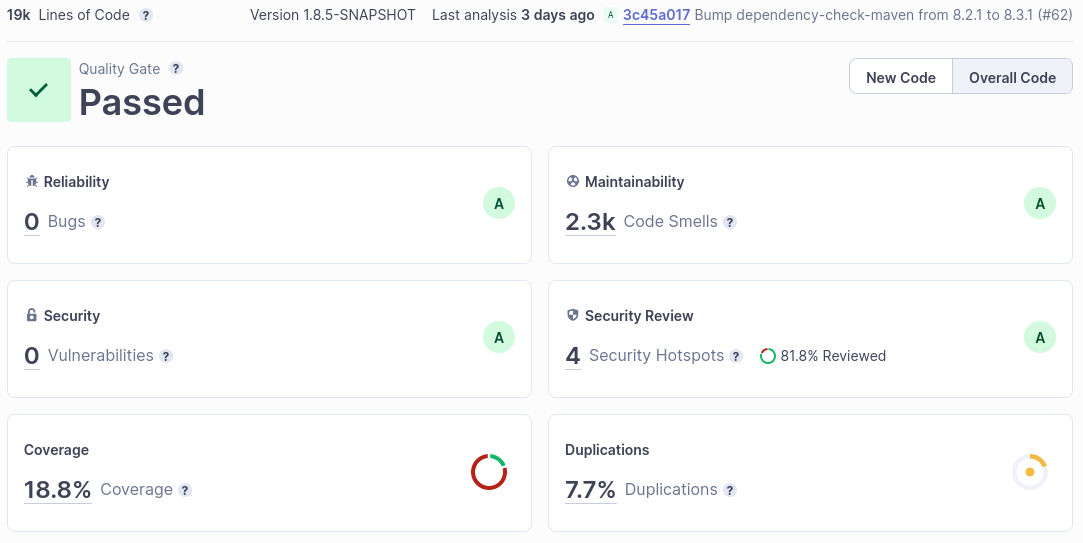
\includegraphics[width=\textwidth]{scfinalc.png}
    \caption{Ergebnis des Bugfixings (Juni 2023)}
    \label{fig:my_sonarf}
\end{figure}


% Highlight 2 der Implementierung
\section{Zentralisierung}
\begin{figure}[ht]
    \centering
    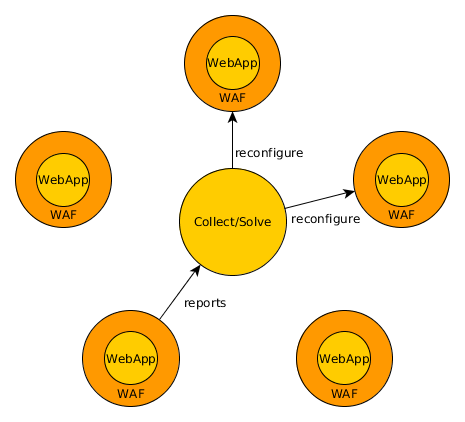
\includegraphics[width=8cm]{central.png}
    \caption{Arbeit der WAFs im Verbund}
    \label{fig:my_verbund}
\end{figure}

\begin{figure}[h]
  \begin{center}
    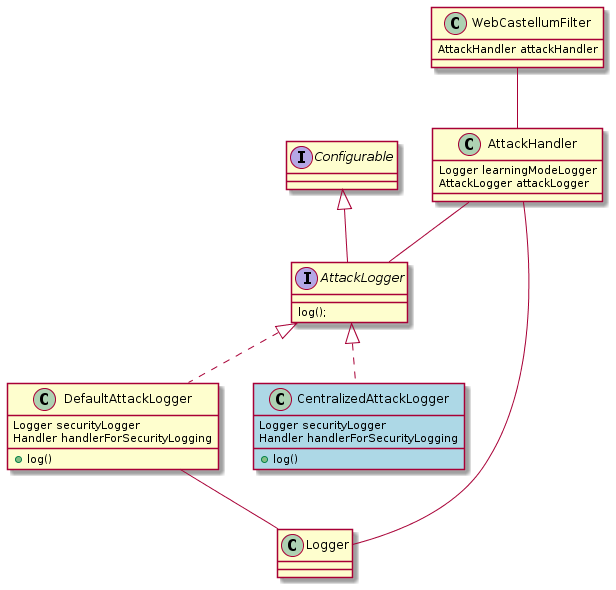
\includegraphics[width=12cm]{classp}
    \caption{Implementierung Nachrichtenversand}
    \label{fig.impversand}
  \end{center}
\end{figure}

\begin{figure}[h]
  \begin{center}
    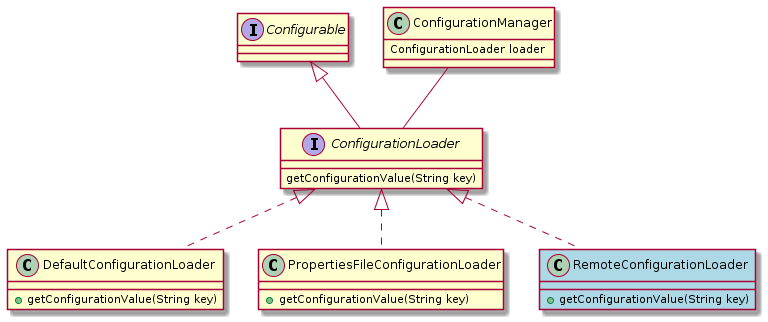
\includegraphics[width=14cm]{configclasses}
    \caption{Implementierung Konfiguration}
    \label{fig.impkonfig}
  \end{center}
\end{figure}



\section{ML-Fähigkeit}

\begin{figure}[h]
    \centering
    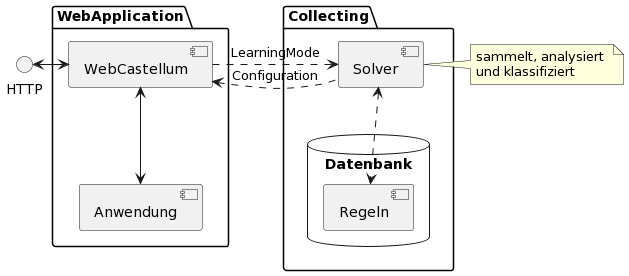
\includegraphics[width=9cm]{webcastellumcentral.png}
    \caption{Komponentendiagramm für zentrale Klassifizierung}
    \label{fig:my_future}
\end{figure}

\section{Lernmodus}

% Highlight des Deployments beim Kunden

% Zusammenfassung: ca. 0,5 Seiten
\section{Zusammenfassung}

% Was haben wir in diesem Kapitel gelernt?
% Wie passt das zur Zielstellung der Arbeit?
% Wie passt das zum nächsten Kapitel?

%Evaluierung (wenn Sie ein System bauen, ca. 10 Seiten)
%  Aufbau der Messumgebung (1-2 Seiten)
%  Ergebnisse und Beobachtungen (3-4 Seiten)
%  Diskussion und Bewertung (3-4 Seiten)
%  Zusammenfassung (ca. 0,5 Seiten)
\chapter{Evaluierung}

\anno{ca. 10 Seiten (4)} %Ref. hat 5

Nachdem im letzten Kapitel hauptsächlich Aspekte der praktischen Umsetzung für das WAF-System erläutert wurden, widmet sich dieses Kapitel der Überprüfung der gemachten Annahmen aus der Zielbeschreibung der Arbeit. Insbesondere die Frage nach möglichst aktuellen bzw. neuen Daten und der damit verbundenen Qualität soll damit beantwortet werden. Dazu werden zuerst die benutzten Werkzeuge und der Testaufbau beschrieben. 

\section{Werkzeuge}
Für den Testaufbau werden einige Grundkomponenten benötigt. 

\subsection{Java Development Kit}
Für den Betrieb der in dieser Arbeit verwendeten Werkzeuge, wie z.B. Anwendungsserver oder Buildtools, ist eine Java-Laufzeitumgebung notwendig. In den lokal ausgeführten Fällen wurde dafür das \emph{Java Development Kit} der Firma Oracle in der Version 17.0.1 verwendet. Die im CI/CD-Build-Cycle ausgeführten Tests und Werkzeuge nutzen hingegen das Eclipse Temurin JDK in der jeweils aktuellsten Version 11.x


\subsection{OWASP\textregistered  Zed Attack Proxy}
\label{ref:zap}

\emph{The world's most widely used web app scanner}\footnote{https://zaproxy.org}\\

Der Zed Attack Proxy (ZAP) wird genutzt um Web Anwendungen auf Sicherheitslücken zu untersuchen. Als sogenannter Proxy befindet sich diese Anwendung zwischen dem Endnutzer bzw. Browser und der zu testenden Anwendung. ZAP bietet dabei zwei verschiedene Anwendungsmodi an. Im passiven Modus \emph{begleitet} ZAP den Nutzer auf seinem Weg durch eine Anwendung und registriert sämtliche IT-sicherheitstechnischen Auffälligkeiten. Der Nutzer klickt sich durch seine Anwendung, ggf. auf einem vorher definierten Weg,  und erhält am Ende eine Übersicht möglicher Angriffswege. Des Weiteren kann dieses Werkzeug zur Aufzeichnung der HTTP-Anfragen und -Antworten genutzt werden\\ Im aktiven Modus übernimmt ZAP selbst die Rolle des Angreifers und versucht Sicherheitslücken automatisch zu finden. \\

Es existieren zahlreiche weitere Tools mit ähnlicher Funktionalität, z.T. auch mit Spezialisierung auf das Testen von Web Application Firewalls. Nennenswerte Beispiele sind \emph{BurpSuite}, \emph{WAFNinja}, \emph{gotestwaf} und \emph{w3af}.  

\subsection{Web Server}

Zur Auslieferung der verwendeten Webapplikationen wird ein Web Server benötigt. Bedingt aus den Anforderungen der zu testenden Webanwendungen und Web Application Firewall muss dieser die Java Servlet Spezifikation implementieren. Bei der Verwendung eines lokalen Web Servers oder in den automatisierten Tests dieser Arbeit wird dabei der Apache Tomcat-Server in der Version 8.5.78 genutzt. Die Ausführung von Anwendungen die auf dem \emph{Spring}-Framework basieren benötigen nicht zwingend einen dedizierten Anwendungsserver, da diese ein integriertes System mit sich bringen (Undertow 2.2.18).

\subsection{WebCastellum}
Bei WebCastellum handelt es sich um eine Web Application Firewall die zum Schutz von Webanwendungen vor allgemeineren Angriffsszenarien entwickelt wurde. Implementiert wurde WebCastellum als ServletFilter, d.h. im Gegensatz zu WAF-Lösungen die als Proxy vor der Anwendung filtern, hätte WebCastellum vollen Zugriff auf alle Informationen die auch der Webanwendung bekannt sind. Erwähnenswert wären hier zum Beispiel der Login- oder Sessionstatus. 


\subsection{Anwendungen}

\subsubsection{PrimeFacesShowcase}

Beim PrimeFaces Showcase\footnote{Download unter https://www.primefaces.org/downloads} handelt es sich um eine Web-Anwendung zur Demonstration der PrimeFaces-Komponenten-Bibliothek. Dabei handelt es sich um eine Sammlung an Komponenten entsprechend der JSF-Spezifikation (JavaServerFaces). Neben der einfachen Darstellung der Komponenten liefert der Showcase auch Quelltext-Beispiele für deren Verwendung. Geht man davon aus dass eine Mehrheit der Entwickler diese Beispiele für eigene Implementierungen nutzt, könnte man schlussfolgern dass zahlreiche Anwendungen sicherheitstechnisch ähnlich reagieren wie der Showcase und dieser stellvertretend hier für den Nachweis genutzt werden kann.\anno{zu kompliziert?} Des weiteren bietet der Showcase die Möglichkeit \emph{alle} Komponenten des Frameworks zu testen.

\subsection{PetStore}

\subsubsection{CargoTracker}

\subsubsection{Spring PetClinic}



\subsubsection{OWASP\textregistered WebGoat}

In Form eines IT-Sicherheitstutorials wurde mit dem WebGoat-Projekt eine \emph{absichtlich, unsichere Anwendung} geschaffen, die es \emph{interessierten Entwicklern erlaubt häufig vorkommende Schwachstellen in Java-basierten Anwendungen} zu testen \cite{owaspgoat}. Da es sich um ein Tutorial handelt sind alles Schwachstellen auch explizit benannt. Ein guter Scanner sollte in diesem Fall auch alle Schwachpunkte auffinden können. 


\section{Aufbau der Testumgebung}
% Aufbau der Messumgebung (1-2 Seiten)
%% Server/Betriebssystem
%% Datensätze
%% Anfragen
%% Systeme/Ansätze gegen die Sie sich vergleichen
%% Wie messen Sie? Methodik und Maßeinheiten?
%% Ist die Messung signifikant?
%% Hypothesen? Was erwarten Sie?

Sämtliche Tests in dieser Arbeit werden nach dem Muster aus Abbildung \ref{fig.pattern} aufgebaut. Ein \glqq Angreifer\grqq versucht einen Angriff auf das \glqq Opfer\grqq. Zum Vergleich folgt auf einen Test ohne \glqq Verteidiger\grqq immer ein gleicher Test mit Verteidiger.

\begin{figure}[bht]
  \begin{center}
    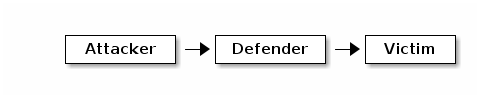
\includegraphics[width=10cm]{pattern}
    \caption{Muster für Tests}
    \label{fig.pattern}
  \end{center}
\end{figure}

\subsection{Attacker}
Angreifer können (handgeschriebene) Tests oder automatisierte Tools sein. Konkret werden in dieser Arbeit folgende Ausprägungen angewandt.

\subsubsection{Der manuelle Angriff}

Ein manueller Angriff ist ein exakt definierter Angriff der manuell ausgeführt wird. Der Ablauf ist dabei exakt in einer (Test-)Spezifikation beschrieben. Häufig existieren diese Tests in Form von Checklisten die vom einem Tester (Mensch) ab zuhaken sind. Mit Werkzeugen wie Selenium existieren auch Möglichkeiten diese Art von Test zu automatisieren. Der hier verwendete Test ruft im Grunde nur ein Formular auf und trägt in ein Textfeld einen mit einer SQl-Injektion versehenen bzw. manipulierten Wert ein. Im Anschluß wird das Formular abgesendet und der Rückgabewert kontrolliert.

\begin{neu}
manuellen Angriff beispielhaft erläutern; ggf. nochmal hinweis auf GrapheneTest (automatisierte Angriff); Hinweis/Übergang zu verschiedenen Beispiel-Datasets bzw. ref aus WAf-a-mole bzgl. verfügbarkeit
\end{neu}


\subsubsection{Der passive Angriff}
Im passiven Angriff wird der bereits aus Abschnitt \ref{ref:zap} bekannte \emph{Zed Attack Proxy} zwischen den Browser und der Webanwendung geschaltet. Im Grunde klickt sich nun ein Anwender durch die Anwendung und der Proxy ließt den Datenverkehr mit. Dabei werden die entdeckten Sicherheitslücken markiert. Um vergleichbare Ergebnisse zwischen den beiden Testläufen (mit und ohne aktiver Web Application Firewall) zu erhalten ist es zwingend erforderlich das beide Testläufe im Ablauf absolut gleich aufgebaut sind. Hierbei hilft beispielsweise die Definition des Testszenarios mittels Ablaufplan. Der Ablaufplan hilft auch bei einer späteren Automatisierung dieses Testvorgehens.

\subsubsection{Der aktive Angriff}
Beim aktiven Angriff übernimmt \emph{ZAP} die volle Kontrolle und sucht (möglichst) selbständig nach potentiellen Schwachstellen in der zugewiesenen Webanwendung. Eine \emph{kleine} Grundkonfiguration ist trotzdem notwendig, beispielsweise um Passworte zu hinterlegen falls ZAP - als Angreifer - auf eine Loginseite trifft. \\\\
\textcolor{bhtGray}{\ding{110} Hinweis} Ist man nicht Eigentümer der Ziel-Webanwendung sollte OWASP ZAPs aktiver Scanmodus nicht genutzt werden!\\


\subsection{Defender}

Hierbei handelt es sich um die zu testende Instanz der WebApplicationFirewall. Gegebenenfalls kann hier natürlich die Konfiguration - je nach Testfall - variieren. Da jedoch eine zentrale Installation im Fokus steht sollte in jedem Fall diese zentrale Instanz getestet werden.
% 3 Fälle -> ohne, defaultconfig, von zentrale gelieferte Konfiguration

\subsection{Victim}

Bei den \glqq\emph{Opfern}\grqq  im Test sollte es sich um zu schützende Anwendungen handeln. Vornehmlich sollte es sich um ein möglichst breit gefächertes Angebot an Anwendungen handeln. Aus zeitlichen Gründen werden in dieser Arbeit jedoch nur die im Grundlagen-Absatz erwähnten Anwendungen, \emph{Primefaces Showcase} und \emph{WebGoat} genutzt. Grundsätzlich könnten aber auch andere Anwendungen für den Testaufbau genutzt werden.\\ 

\subsection{TestMatrix}
Grundsätzlich besteht Bedarf möglichst viele Szenarien im Test abzudecken. Hierfür wird die in Tabelle \ref{tab:testplan} als Grundgerüst verwendet. Möglichst alle Angreifer sollten jeweils jedes Opfer angreifen. Mit steigender Anzahl an Opfern bzw. Tätern würde sich die Matrix entsprechend erweitern.


\begin{table}[h]
    \centering
    \begin{tabular}{cccc} 
      \toprule
    \textbf{Testlauf} & \textbf{Angreifer} & \textbf{Verteidiger} & \textbf{Opfer} \\ 
     \midrule
     1 & manuell & - & PF showcase\\
     2 & manuell & WebCastellum & PF showcase \\
     3 & ZAP (passiv) & - & PF showcase\\
     4 & ZAP (passiv) & WebCastellum & PF showcase \\
     5 & ZAP (aktiv) & - & PF showcase\\
     6 & ZAP (aktiv) & WebCastellum & PF showcase \\
     7 & manuell & - & WebGoat \\ 
    8 & manuell & WebCastellum & WebGoat \\
    9 & ZAP (passiv) & - & WebGoat \\ 
    10 & ZAP (passiv) & WebCastellum & WebGoat \\
    11 & ZAP (aktiv) & - & WebGoat \\ 
    12 & ZAP (aktiv) & WebCastellum & WebGoat \\
   \bottomrule
    \end{tabular}
    \caption{Testplan}
    \label{tab:testplan}
\end{table}

% Ergebnisse und Beobachtungen (3-4 Seiten)
\section{Ergebnisse und Beobachtungen}

% Beschreibung der Ergebnisse
% Diagramme
% Darstellen von Zusammenhängen

\anno{Tabellenwert! webgoat is spring ML lernen}

%lohnt es sich Training mit altem und neuen Datensatz zu testen? Zeit?

Die Ergebnisse aus den Tests (nach der spezifizierten Testmatrix) zeigen eine eindeutige Verbesserung durch Nutzung der Web Application Firewall. 

\begin{table}[h]
    \centering
    \begin{tabular}{cccccc} 
      \toprule
    \textbf{Testlauf} & \textbf{Angreifer} & \textbf{Verteidiger} & \textbf{Opfer} & \textbf{Schwachstellen} & \textbf{Verbesserung(in \%)} \\ 
     \midrule
     1 & manuell & - & PF showcase & 3 &\\
     2 & manuell & WebCastellum & PF showcase & 1 & 66\\
     3 & ZAP (passiv) & - & PF showcase & 16 &\\
     4 & ZAP (passiv) & WebCastellum & PF showcase & 2 & 87.5 \\
     5 & ZAP (aktiv) & - & PF showcase & 56 & \\
     6 & ZAP (aktiv) & WebCastellum & PF showcase & 20 & 64.3\\
     7 & manuell & - & WebGoat & 10 & \\ 
    8 & manuell & WebCastellum & WebGoat & 3 & 70 \\
    9 & ZAP (passiv) & - & WebGoat & 25 & \\ 
    10 & ZAP (passiv) & WebCastellum & WebGoat & 12 & 50\\
    11 & ZAP (aktiv) & - & WebGoat & 34 & \\ 
    12 & ZAP (aktiv) & WebCastellum & WebGoat & 14 & 59 \\
   \bottomrule
    \end{tabular}
    \caption{Ergebnisse}
    \label{tab:tes1tergebnisse}
  \end{table}

  Tabelle \ref{tab:tes1tergebnisse} gibt einen Überblick über die allgemeine Frage ob Angriffe verhindert werden können. Grundsätzlich verbessert der Einsatz einer WAF die IT-Sicherheit signifikant. Die zweite Tabelle verdeutlicht die Ergebnisse nochmals anhand der einzelnen Kategorien.

\begin{table}[h]
    \centering
    \begin{tabular}{cccccc} 
      \toprule
    \textbf{Testlauf} & \textbf{SQLi} & \textbf{CSRF} & \textbf{XMLi} & \textbf{sonstige} & \textbf{gesamt} \\ 
     \midrule
     1 & 2 & 1 &  &  & 3\\
     2 &   & 1 &  &  & 1\\
     3 & 6 & 5 &  & 5 & 16\\
     4 &   & 1 &  & 1  & 2 \\
     5 & 22 & 9 & 7 & 8& 56\\
     6 &  & 7 & 5 & 8 & 20 \\
     7 & 7 & 3 &  &  &  10  \\ 
    8 &  & 3 &  & & 3  \\
    9 & 11 & 5 &  & 9 & 25 \\ 
    10 &   & 5 &  & 7  & 12 \\
    11 & 17 & 8 &  & 9 & 34  \\ 
    12 &  & 8 &  & 6 & 14 \\
   \bottomrule
    \end{tabular}
    \caption{Ergebnisse}
    \label{tab:tes2tergebnisse}
\end{table}

Betrachtet man Tabelle \ref{tab:tes2tergebnisse} fällt auf das die Wirksamkeit der Firewall insbesondere im Fall von SQL-Injections (SQLi) gegeben ist. Nach Einsatz der Firewall wurden alle vorher erkannten Schwachstellen geschlossen bzw. eine Ausnutzung der Schwachstelle verhindert. Beide Anwendungen beinhalten eine oder mehrere Schwachpunkte im Bereich Cross-Site-Request-Forgery (CSRF). Obwohl die WAF-Software einen derartigen Schutzmechanismus beinhaltet scheint dieser nur im \emph{Primefaces Showcase} zum Teil zu wirken. Für die \emph{WebGoat}-Anwendung scheint dieser jedoch wirkungslos zu sein.


% Diskussion und Bewertung (3-4 Seiten)
\section{Bewertung}

% Wurden Sie überrascht?
% Stimmten die Hypothesen?
% Sind sie besser, anders als das andere System?
% wichtigster Erkenntnisgewinn?
% Anwendbarkeit Szenario?


% Zusammenfassung: ca. 0,5 Seiten


\section{Zusammenfassung}

% Was haben wir in diesem Kapitel gelernt?
% Wie passt das zur Zielstellung der Arbeit?
% Wie passt das zum nächsten Kapitel?

%Zusammenfassung und Ausblick (5 Seiten)
%  Zusammenfassung
%  Ausblick
\chapter{Zusammenfassung und Ausblick}

\anno{5 Seiten} %Ref. 3

% Zusammenfassung

% Ausblick
\section{Ausblick}

\begin{neu}
  Nacharbeit Überführung der Evaluation als arquillian test?!
  Bereitstellung als (neuere) WebCastellum Version und Bereitstellung des zentralen Sammelpunktes.
\end{neu}

% https://www.dev-insider.de/wie-angreifbar-ist-webgoat-wirklich-a-7a385bc1e48bb04b7fdc9034029555e1/


\begin{appendix}
  %%
%% Beuth Hochschule für Technik --  Abschlussarbeit
%%
%% Anhang
%%
%%%%%%%%%%%%%%%%%%%%%%%%%%%%%%%%%%%%%%%%%%%%%%%%%%%%%%%%%%%%%%%%%%%%%


\chapter{Angehängtes: Die Dateien des Pakets}

\subsection*{Tabellen}

\begin{table}[h]
  \centering
  \resizebox{\textwidth}{!}{
    \begin{tabular}{|c | c | c | c |} 
 \hline
      \textbf{WAF Name} & \textbf{Hersteller} & \textbf{WAF Name} & \textbf{Hersteller} \\
      \hline
      ACE XML Gateway & Cisco & FirePass & F5 Networks\\
      Airlock & Phion/Ergon & FortiWeb & Fortinet\\
      Alert Logic & Alert Logic & GoDaddy Website Protection & GoDaddy\\
      AliYunDun & Alibaba Cloud Computing & Huawei Cloud Firewall & Huawei\\
      AnYu & AnYu Technologies & HyperGuard & Art of Defense\\
      AppWall & Radware & Imunify360 & CloudLinux\\
      Armor Defense & Armor & Incapsula & Imperva Inc.\\
      ArvanCloud & ArvanCloud & ISA Server & Microsoft\\
      ASP.NET Generic & Microsoft & Janusec Application Gateway & Janusec\\
      ASPA Firewall & ASPA Engineering Co. & Kona SiteDefender & Akamai\\
      Astra & Czar Securities & KS-WAF & KnownSec\\
      AWS Elastic Load Balancer & Amazon & LimeLight CDN & LimeLight\\
      AzionCDN & AzionCDN & Oracle Cloud & Oracle\\
      Azure Front Door & Microsoft & ModSecurity & SpiderLabs\\
      Barracuda & Barracuda Networks & NetContinuum & Barracuda Networks\\
      Bekchy & Faydata Technologies Inc. & NetScaler AppFirewall & Citrix Systems\\
      Beluga CDN & Beluga & NullDDoS Protection & NullDDoS\\
      BinarySec & BinarySec & PentaWAF  & Global Network Services\\
      BitNinja & BitNinja &   PT Application Firewall & Positive Technologies\\
      BlockDoS & BlockDoS &   Profense  & ArmorLogic\\
      Bluedon & Bluedon IST &   Qcloud   & Tencent Cloud\\
      CacheWall & Varnish &   RequestValidationMode   & Microsoft\\
      CacheFly CDN & CacheFly &   Sabre Firewall     & Sabre\\
      Comodo cWatch & Comodo CyberSecurity &   eEye SecureIIS & BeyondTrust\\
      CdnNS Application Gateway & CdnNs/WdidcNet &   SecuPress WP Security  & SecuPress\\
      ChinaCache Load Balancer & ChinaCache &   SecureSphere  & Imperva Inc.\\
      Chuang Yu Shield & Yunaq &   SEnginx       & Neusoft\\
      Cloudbric & Penta Security &   SiteGuard  & Sakura Inc.\\
      Cloudflare & Cloudflare Inc. &   SonicWall   & Dell\\
      Cloudfloor & Cloudfloor DNS &   UTM Web Protection              & Sophos\\
      Cloudfront & Amazon &   SquidProxy IDS   & SquidProxy\\
      CrawlProtect & Jean-Denis Brun &   Tencent Cloud Firewall   & Tencent Technologies\\
      DataPower & IBM &   Teros   & Citrix Systems\\
      DenyALL & Rohde+Schwarz CyberSecurity &  Trafficshield  & F5 Networks\\
      Distil & Distil Networks &   Varnish        & OWASP\\
      DotDefender & Applicure Technologies &   WebSEAL  & IBM\\
      DynamicWeb Injection Check & DynamicWeb &   XLabs Security WAF   & XLabs\\
      BIG-IP AppSec Manager & F5 Networks &   ZScaler & Accenture\\
      BIG-IP AP Manager & F5 Networks & & \\
      Fastly & Fastly & & \\
      \hline
      
      
\end{tabular}}
\caption{Auszug WAFw00f Plugins(aus https://github.com/EnableSecurity/wafw00f)}
\medskip
\small
WAFw00f ist ein Werkzeug zur Identifikation von WAFs und die Liste der Plugins gleichzeitig eine Liste der WAF-Produkte die WAFw00f erkennt.
\label{tab:my_wafwoof}
\end{table}

\begin{table}[h]
  \centering
%  \resizebox{\textwidth}{!}{
  \begin{tabular}{|l | p{7cm} |}
    \hline
    \textbf{Name} & \textbf{Beschreibung} \\
    \hline
    gotestwaf & tool for API and OWASP attack simulation \\
    BurpSuite & vulnerability scanning, penetration testing, and web app security platform\\
    identYwaf & identification tool that can recognize web protection \\
    lightbulb-framework & framework for auditing web application firewalls \\
    OWASP Zed Attack Proxy & the world's most widely used web app scanner \\
    Paros Proxy & A Java based HTTP/HTTPS proxy for assessing web application vulnerability.\\
    sqlmap & testing tool that automates SQL injection\\
    w3af & Web Application Attack and Audit Framework\\
    weka & Waikato Environment for Knowledge Analysis - collection of ML algorithms for data mining tasks\\
    waf-brain & WAF - the Machine-Learning-Deep-Learning-Way\\
    waf-bypass & open source tool to analyze the security of an WAF\\
    WAFNinja &  WAFNinja is a tool which contains two functions to attack Web Application Firewalls. \\
    wafw00f & allows one to identify and fingerprint Web Application Firewall products\\
    \hline
    % \end{tabular}}    
  \end{tabular}
  
  \caption{Übersicht Werkzeuge}
  \medskip
  \small
  (Die Beschreibung der Werkzeuge wurde den jeweiligen Internetpräsenzen entnommen)
  \label{tab:my_tools}
\end{table}

\begin{table}[h]
  \centering
  \begin{tabular}{|l|}
    \hline
    Eclipse CargoTracker \\
    J2EE PetStore \\
    Spring PetClinic \\
    JBoss QuickStarts (KitchenSink) \\
    PrimeFaces Showcase \\
    \hline
  \end{tabular}
  \caption{Übersicht Demo Anwendungen}
  \label{tab:exampleapp}
\end{table}

\begin{table}[h]
  \centering
  \begin{tabular}{|l|}
    \hline
    JavaVulnerableLab \\
    Marathon\\
    VulnarableSpring \\
    OWASP Mutillidae II \\
    OWASP WebGoat \\
    \hline
  \end{tabular}
  \caption{Übersicht Absichtlich angreifbare Anwendungen}
  \label{tab:vulnapp}
\end{table}

\begin{table}[h]
  \centering
  \begin{tabular}{|l|}
    \hline
    \textbf{Feature Name} \\
    \hline
    Length of the request \\
    Length of the path \\
    Length of the arguments \\
    Length of the header \glqq\emph{Accept}\grqq \\
    Length of the header \glqq\emph{Accept-Encoding}\grqq \\
    Length of the header \glqq\emph{Accept-Charset}\grqq \\
    Length of the header \glqq\emph{Accept-Language}\grqq \\
    Length of the header \glqq\emph{Cookie}\grqq \\
    Length of the header \glqq\emph{Content-Length}\grqq \\
    Length of the header \glqq\emph{Content-Type}\grqq \\
    Length of the Host \\
    Length of the header \glqq\emph{Referer}\grqq \\
    Length of the header \glqq\emph{User-Agent}\grqq \\
    Method identifier\\
    Number of arguments\\
    Number of letters in the arguments\\
    Number of digits in the arguments\\
    Number of special char in the arguments\\
    Number of other char in the arguments\\
    Number of letters in the path\\
    Number of digits in the path\\
    Number of special char in the path\\
    Number of other char in the path\\
    Number of cookies\\
    Minimum byte value in the request\\
    Maximum byte value in the request\\
    Number of distinct bytes\\
    Entropy\\
    Number of keywords in the path\\
    Number of keywords in the arguments\\
    \hline
  \end{tabular}
  \caption{Names of 30 expert knowledge features that are considered relevant for the detection of web attacks for the CSIC dataset (s. Tabelle 5.2. in \cite{Giménez2015})}
  \label{tab:tgfeatures}
\end{table}

\end{appendix}
%%%%%%%%%%%%%%%%%%%%%%%%%%%%%%%%%%%%%%%%%%%%%%%%%%%%%%%%%%%%%%%
%% Literaturverzeichnis

\clearpage\newpage
\addcontentsline{toc}{chapter}{Literatur- und Quellenverzeichnis}
\bibliographystyle{myapalike}
\bibliography{bhtThesis}

\end{document}
